\documentclass[11pt,twoside]{article}
\addtolength{\textwidth}{0.5in}
\usepackage{epsfig,amsfonts,color}
\usepackage{amsmath}
\usepackage{multirow}
\bibliographystyle{plain}
\usepackage{amssymb, palatino, geometry,url}
\usepackage{algorithmic}
\usepackage[noresetcount,lined,boxed]{algorithm2e} % ... for algorithms
\usepackage[colorlinks=true,linkcolor=blue,citecolor=blue,urlcolor=blue]{hyperref}
\geometry{letterpaper,
          left       = 0.9in,
          right      = 0.9in,
          top        = 0.9in,
          bottom     = 0.9in}
\linespread{1.2}

\usepackage{fancyhdr}
\usepackage{enumerate}
\usepackage{float}
\usepackage{subcaption}
\usepackage{graphicx}
\usepackage{caption}
\newcommand{\twopart}[4]
{
	\left\{
		\begin{array}{ll}
			#1 & \mbox{ } {\textrm{#2}} \\
			#3 & \mbox{ } {\textrm{#4}}
		\end{array}
	\right.
}

\newcommand{\N}{\mathbb{N}}
\newcommand{\Z}{\mathbb{Z}}
\newcommand{\Q}{\mathbb{Q}}
\newcommand{\R}{\mathbb{R}}
\usepackage{placeins}
\usepackage{lineno}
%\linenumbers
\usepackage{array}
\newcolumntype{L}[1]{>{\raggedright\let\newline\\\arraybackslash\hspace{0pt}}m{#1}}
\newcolumntype{C}[1]{>{\centering\let\newline\\\arraybackslash\hspace{0pt}}m{#1}}
\newcolumntype{R}[1]{>{\raggedleft\let\newline\\\arraybackslash\hspace{0pt}}m{#1}}
\usepackage{graphicx}

\begin{document}

\title{Analysis of Multi-Scale Energy Markets using Stochastic Optimization Techniques}

\author{\textbf{\textit{ISyE 719 Course Project}}\\ \\Apoorva Sampat and Ranjeet Kumar\\
 {\small Department of Chemical and Biological Engineering}\\
 {\small \;University of Wisconsin, 1415 Engineering Dr, Madison, WI 53706, USA}}
\date{}
\maketitle

\begin{abstract}
Electricity markets operate at multiple timescales (from hours to milliseconds) to ensure that supply and demands are matched in real time. These markets involve uncertainties because future electricity prices and demands are unknown at the time of decision-making, e.g. energy sale and purchase commitments by generators. We use stochastic programming techniques to study flexibility and economic opportunities provided by a battery in these markets, namely day-ahead (1-hour timescale) and real-time (5-minute timescale) markets. In this work, we consider uncertainty only in electricity loads and determine optimal participation strategies using methods like extensive form with sample average approximation, receding horizon scheme and dual dynamic programming. We also determine bounds on expected policy costs by using perfect information and two-stage approximation (with restriction on states). We compare the costs of participation in exclusively in day-ahead market and both day-ahead and real-time markets. Our results show that market participation only in day-ahead energy markets can significantly reduce economic flexibility as compared to participating in both levels of markets.
\end{abstract}


\section{Introduction}
A diverse set of energy systems such as generators, batteries, wind turbines and flywheels can participate in electricity markets. This participation is governed by rules set by ISOs (Independent System Operators) such as California ISO (CAISO), Pennsylvania-New Jersey-Maryland (PJM) Interconnection and Midcontinent ISO, under whose jurisdiction the market falls. The markets are structured at multiple time levels, namely day-ahead (hourly market commitments) and real-time markets (commitments ranging from minutes to seconds). In day-ahead markets (DAM) the electricity is traded in intervals of 1 hour with the prices being constant in each interval of 1 hour and varying with intervals. real-time markets (RTM), on the other hand, can have varying timescales depending on the ISO operating it. For example, in California markets (CAISO) the real-time markets are operated at two timescales, a 15-minute timescale which is commonly called as quarter-hourly market (QHM) and a 5-minute timescale which is called as real-time market (RTM), although both are categorized under the real-time market operations by CAISO. The real-time market is a spot market in which utilities can buy power to meet the last few increments of demand not covered in their day-ahead schedules. It is also the market that secures energy reserves, held ready and available for ISO use if needed, and the energy needed to regulate transmission line stability \footnote{http://www.caiso.com/market/Pages/MarketProcesses.aspx}.The frequency of energy price variation is different for day-ahead and real-time markets (Figure \ref{eprices}). The real-time market is more volatile, and at times the prices can even go negative here. This provides an opportunity to the building-battery system to buy electricity at negative price and meet its load demands. The fast dynamics of battery helps it to capture these spikes in prices and maximize its revenue potential. 

\begin{figure}[h!tp]
\centering
\begin{subfigure}[b]{0.32\textwidth} 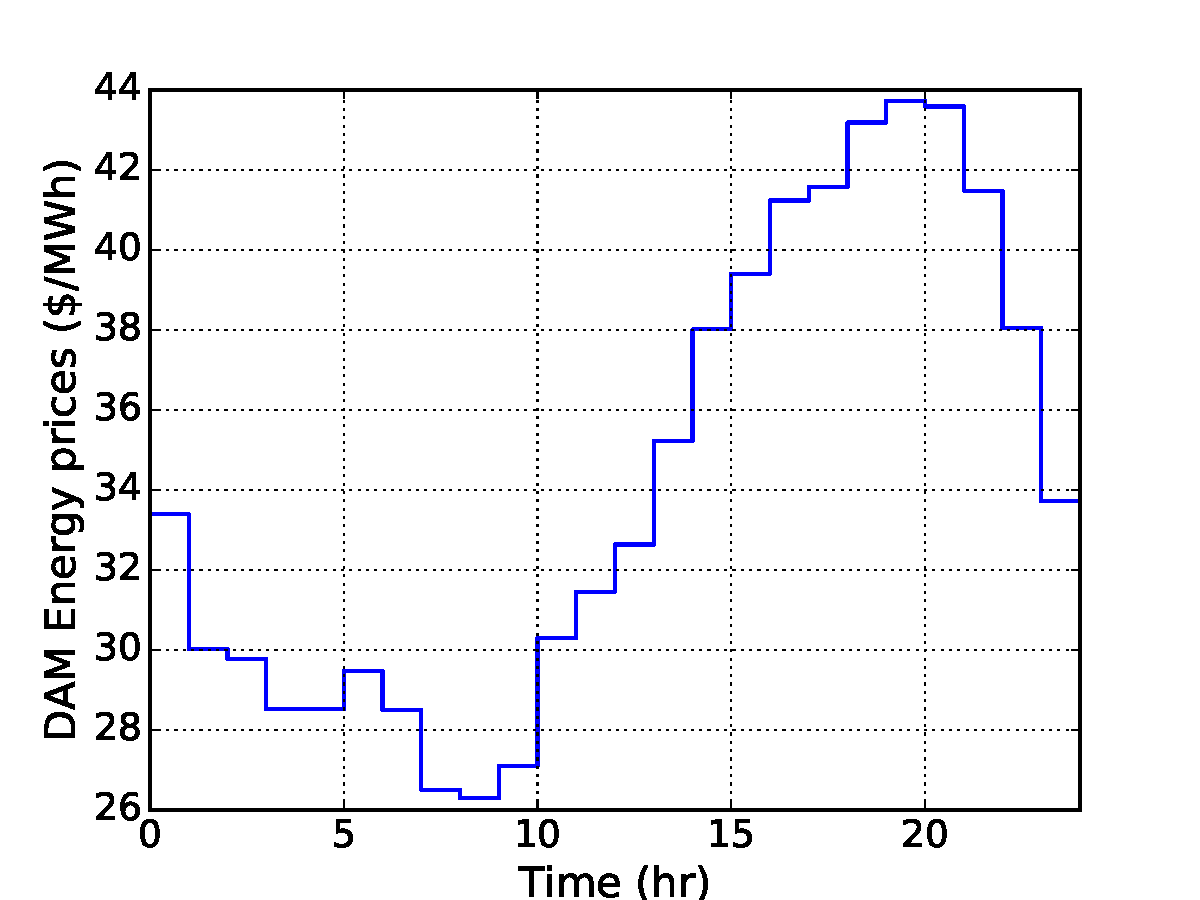
\includegraphics[width=\textwidth]{Figures/damprices.pdf} \caption{Day-ahead market}\label{damprices} \end{subfigure} \hfill
\begin{subfigure}[b]{0.32\textwidth} 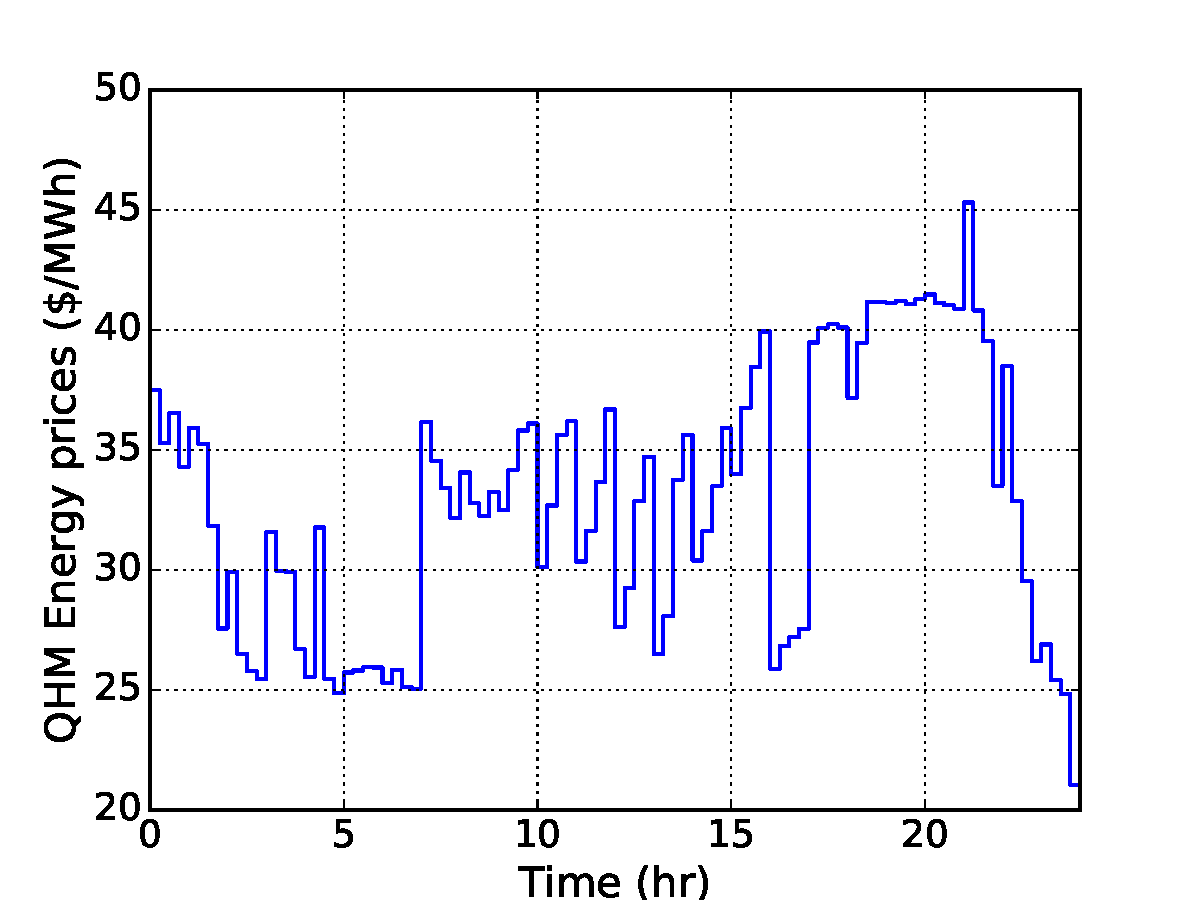
\includegraphics[width=\textwidth]{Figures/qhmprices.pdf} \caption{Quarter-hourly market}\label{qhmprices} \end{subfigure} \hfill
\begin{subfigure}[b]{0.32\textwidth} 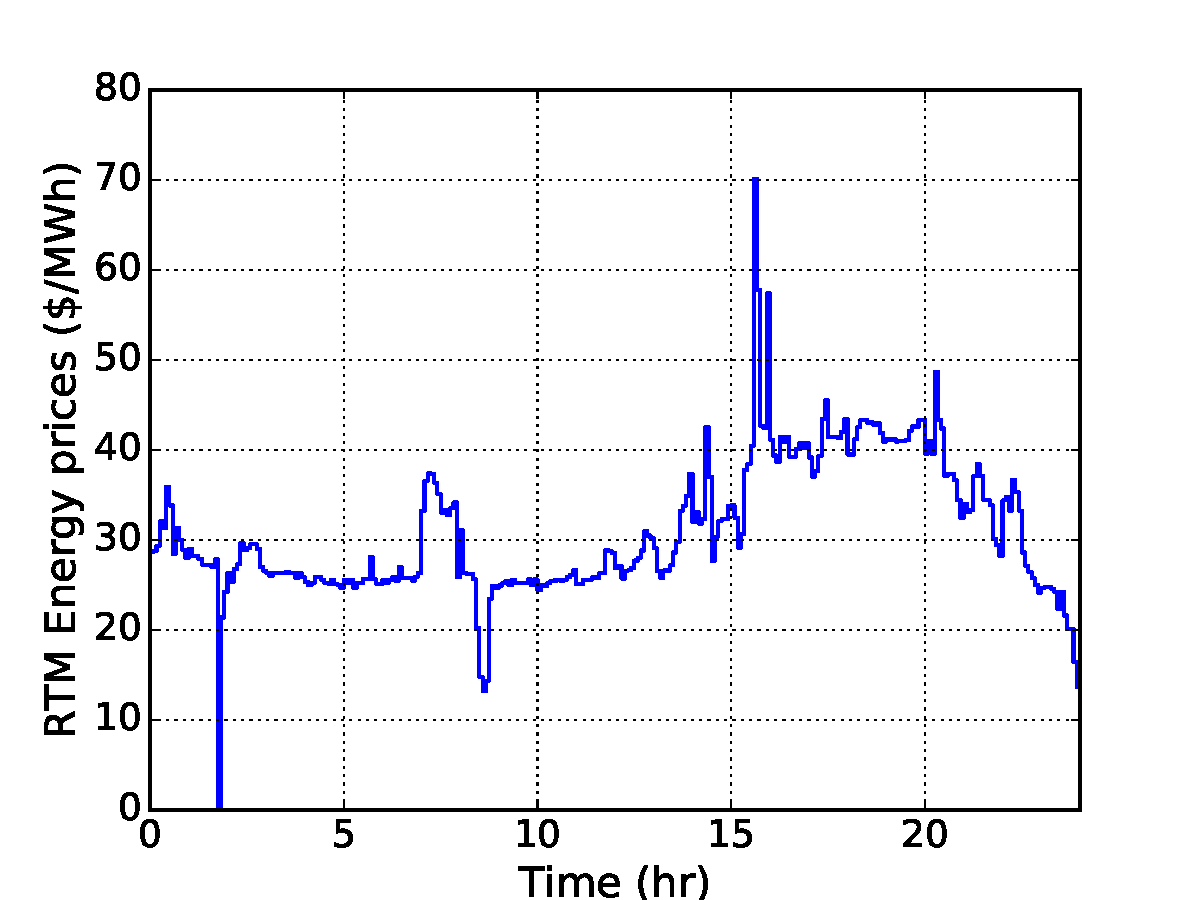
\includegraphics[width=\textwidth]{Figures/rtmprices.pdf} \caption{Real-time market}\label{rtmprices}\end{subfigure} \hfill
\caption{Energy prices for a day in the markets in California. The day-ahead market (DAM) prices vary at 1-hour timescale, the quarter-hourly market (QHM) prices are at 15-minute timescale, the real-time market (RTM) prices are at 5-minute resolution.}\label{eprices}
\end{figure}

Apart from price variations, the introduction of more renewable power sources in the grid such as wind and solar energy, there are greater variations and uncertainties in the net load as well. Since these sources depend on intermittent conditions such as weather, they introduce slow dynamics to the grid. Thus systems with faster dynamic responses such as battery and building systems are becoming increasingly important to balance these fluctuations and provide dynamic flexibility to the power grid. Also, factors such as transmission losses, generation cost and congestion affect the value of products (energy, regulation, spinning, non-spinning reserves) offered at different timescales. These fluctuations being inherently uncertain, determining the optimal participation policy requires analysis using stochastic optimization techniques.

\section{Problem Definition and Decision-Making Setting}\label{sec:setting}
We consider a rechargeable Li-ion battery with a building that is inter-connected to the power grid for providing electricity services. Electricity services imply that batteries can provide power to or draw power from the grid. In our current setting, we do not consider participation in regulation or other ancillary services. The operator of the power grid (ISO) compensates the battery owners for the electricity services provided. The goal for the battery owners is to maximize the revenues generated by providing services to the grid and at the same time meeting the load demands from building. We consider battery and building as one system (building-battery system) and any unmet load demand from the building is penalized with the corresponding electricity price in real-time market.\\
\begin{figure}[h!]
\begin{center}
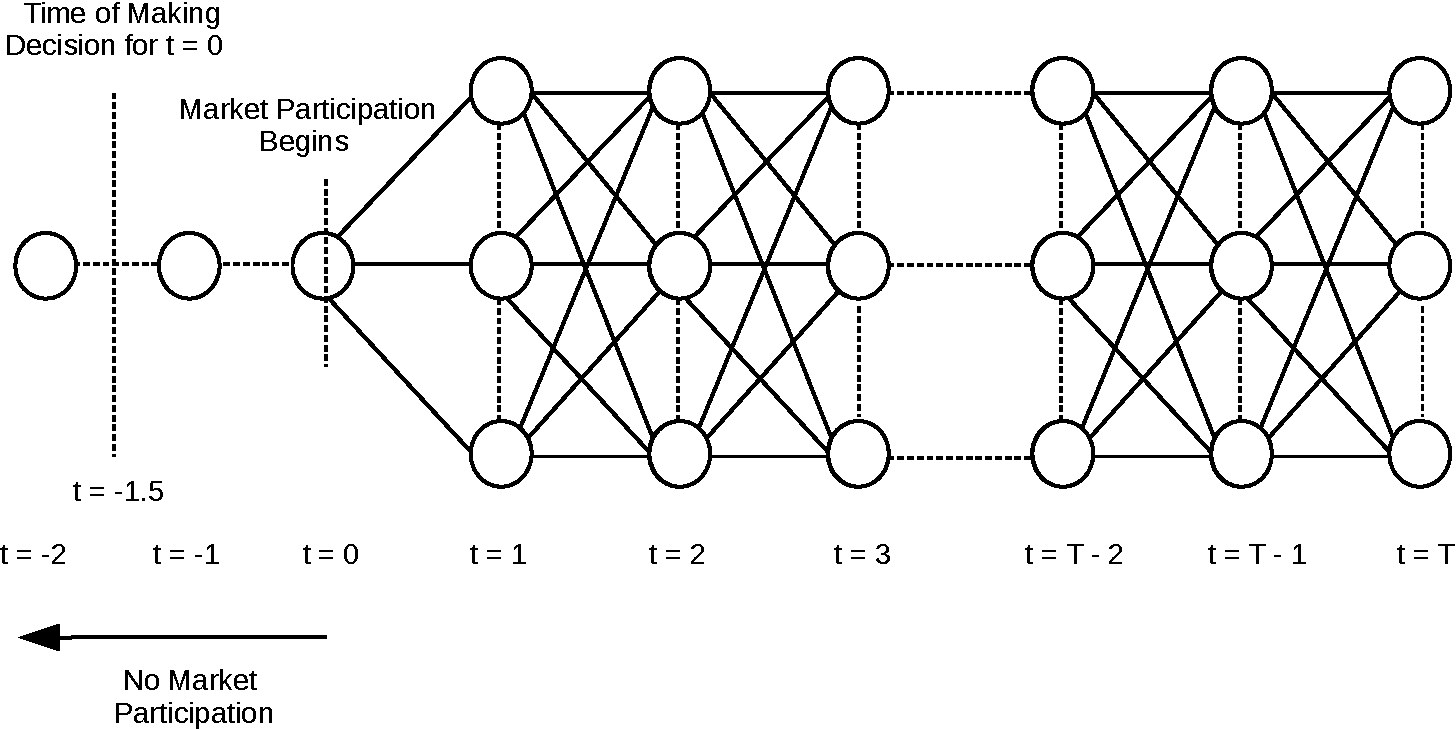
\includegraphics[width=5in]{Figures/scenario_tree-crop.pdf} \caption{Scenario tree at the beginning of market participation}\label{fig:scenario_tree}\end{center}
\end{figure}
We generate a compact scenario tree consisting of 12 sub-intervals between any two hours. One scenario represents a load profile in these 12 subintervals. The participation in market begins at time t = 0 hrs (Figure \ref{fig:scenario_tree}) and decisions can be made latest till 1.5 hrs before any hour (according to market rules set by ISO). Thus our decision making starts at -1.5 hrs (as shown in Figure \ref{fig:scenario_tree}) and our participation begins at t = 0 hrs.   

We divide an annual dataset for electricity loads (available over 5-minute intervals) into 52 subsets of weekly load profiles, i.e 2016 intervals of 5-minute each. This division of data helps in capturing the different load profiles over the weekdays and the weekend. We then use these 52 weekly profiles to generate sample scenarios for our computational experiments (Section \ref{sec:exp}). Since the loads are correlated between time intervals, we formulate a multivariate normal distribution for weekly loads using a mean vector and a covariance matrix. The mean vector (of size 2016 x 1) is the mean of the 52 datasets, but the covariance matrix (of size 2016 x 2016) calculated directly from the 52 datasets cannot be used, since its rank can at most be 52. So we use the Ledoit-Wolf Covariance Estimator \cite{ledoit2004well} (to tackle rank deficiency) for estimating a full rank covariance matrix. We generate 50 samples of load profiles (Figure \ref{fig:loads_scenarios}) for a week using the mean and covariance matrix obtained. 
\begin{figure}[h!]
\begin{center}
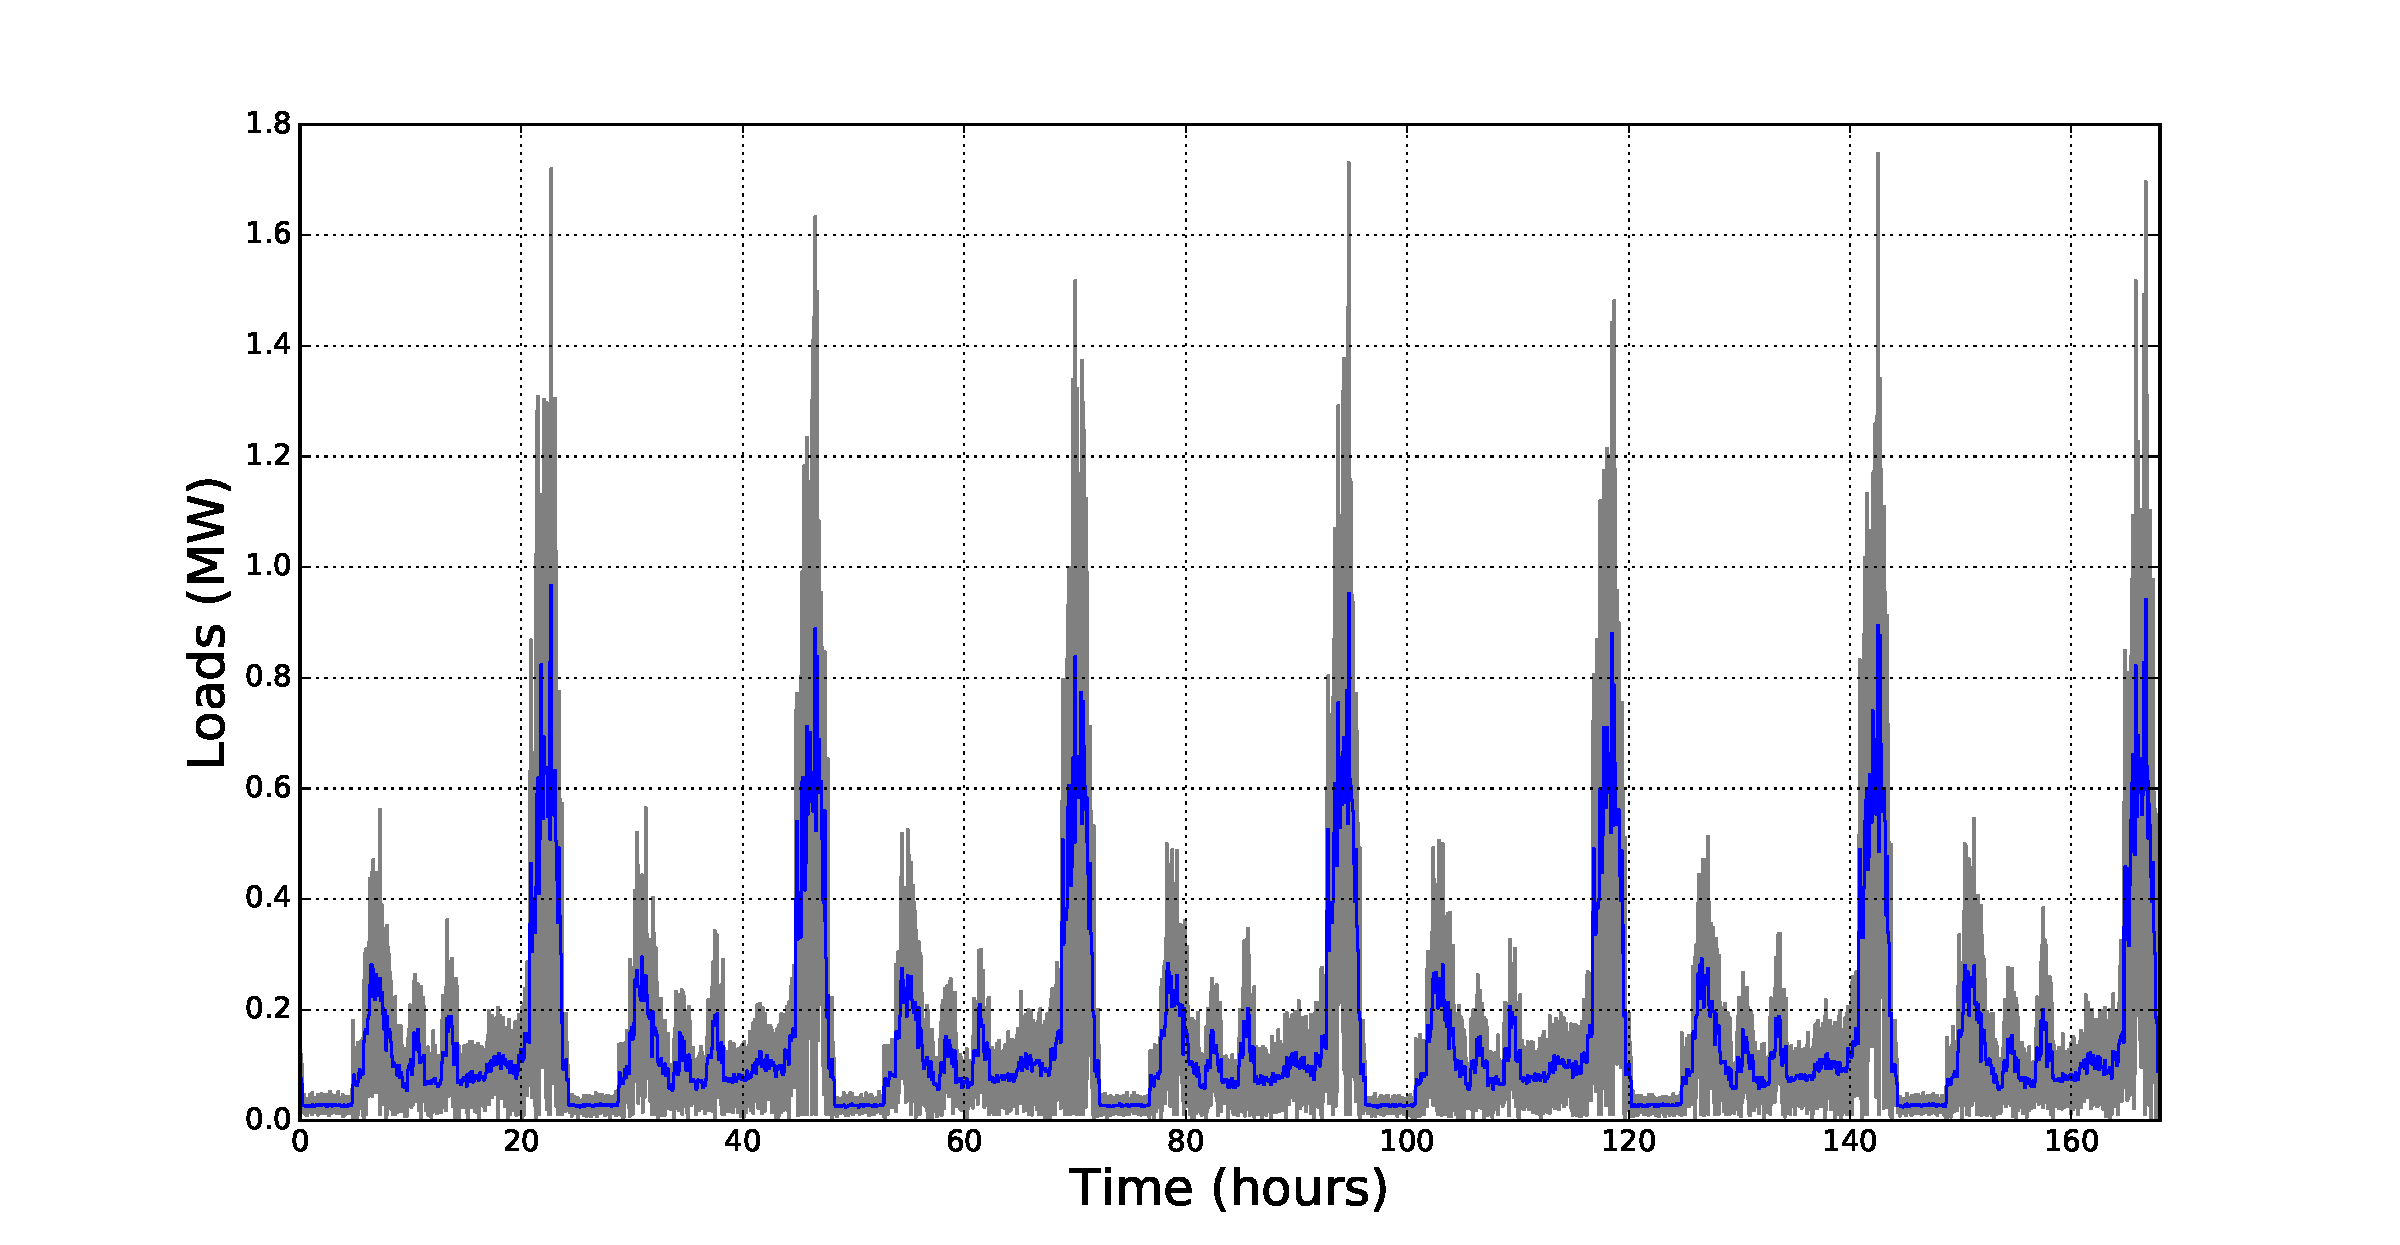
\includegraphics[width=5in]{Figures/Plots/fullproblem_stoch/loads_scenarios.pdf} \caption{Load scenarios for a week. Grey region corresponds to all possible scenarios for the loads while the blue curve represents the mean scenario.}\label{fig:loads_scenarios}\end{center}
\end{figure}
\FloatBarrier
In this work, we assume uncertainty only in the load demands and consider the day-ahead market participation to be first stage decision while real-time market decisions are treated as recourse. Since it involves a multi-period decision-making, it is a multi-stage stochastic programming problem. We first explore the two-stage approximation of the multi-stage stochastic problem and then study the multi-stage approaches for this problem. The goals of this work include:
\begin{itemize}
\item Formulate an extensive form stochastic program for the problem and using two-stage approximation and sample average approximation
\begin{itemize}
\item investigate the economic potential of participating in various markets within a stochastic programming setting, i.e. compare expected revenue from different markets and explore the benefits of participating in both real-time and day-ahead markets.
\item estimate upper and lower bound estimations using perfect information and two-stage approximation (restriction)
\end{itemize}
\item Employ different multi-stage stochastic optimization solution methods and compare their performance. The methods compared are:
\begin{itemize}
\item Stochastic dual dynamic programming (SDDP)
\item Receding horizon 
\end{itemize}
\end{itemize}

\section{Optimization Model for Building-Battery System}\label{sec:model}
\subsection{Deterministic Setting}\label{subsec:deterministic}
First, we formulate an optimization problem to minimize the cost (or maximize revenue) for the building-battery system operating in the electricity market in a deterministic setting assuming no uncertainty in any of the market and demand quantities. In this formulation, the building-battery system participates in the market at two timescales, hourly and 5-minute intervals. Since the price and load signals are discrete, real-time prices and loads available at 5-minute intervals and day-ahead prices at hourly intervals, we make the zero-order hold assumption, i.e. these time-varying signals are constant within an interval of corresponding duration of their timescale. We also assume that the energy stored in the battery before beginning of market participation is fixed at $E_{0}$. The building-battery system is illustrated with a schematic diagram in Figure \ref{fig:system}.

With these assumptions, we develop the optimization problem formulation for the system which is described below.
\subsubsection{Sets used in the model}
\begin{center}
$\mathcal{T_R} := \{1,..,n_{\textrm{rtm}}\}$\\$ \mathcal{T_D} :=  \{1,..,n_{\textrm{dam}}\}$
\end{center}
Here, $\mathcal{T_R}$ is the set of time indices corresponding to each 5-minute subintervals in the real-time market within each hour, so $n_{rtm}=12$. $\mathcal{T_D}$ is the set of time indices corresponding to the hourly intervals of the day-ahead market. $n_\text{dam}$ can be chosen appropriately for any number of hours we plan to schedule the market participation policy for the building-battery system.
\subsubsection{Time discretization used in the model}
A time instance for a day-ahead market variable in the model is represented by only the index $k$ ($k \in \mathcal{T_D}$) which corresponds to the interval between hours $k-1$ and $k$. On the other hand, a time instance for a real-time variable in the model is represented by index $(i,k)$, where $i \in \mathcal{T_R}$ and $ k \in \mathcal{T_D}$. The indices $i$ and $k$ in a time instance $(i,k)$ for a real-time variable correspond to the end of the respective 5-minute subinterval. For example, the time instance ($5,7$) corresponds to the end of the subinterval between $4^{\text{th}}$ and $5^{\text{th}}$ subintervals within the $7^\textrm{th}$ hour. 

So, if a variable or time-varying parameter is indexed by only one index $k$ it implies that it varies at hourly intervals and belongs to the day-ahead market, whereas a variable or time-varying parameter indexed by $(i,k)$ is a real-time variable. 

The time discretization and zero-order hold have been illustrated for the battery power in real-time and day-ahead markets in Figure \ref{fig:discretization}, in which the step-curve in red is showing the variation and indexing of a day-ahead variable (power) and the blue step-curve shows that for a real-time variable.
\begin{figure}[h!]
\begin{center}
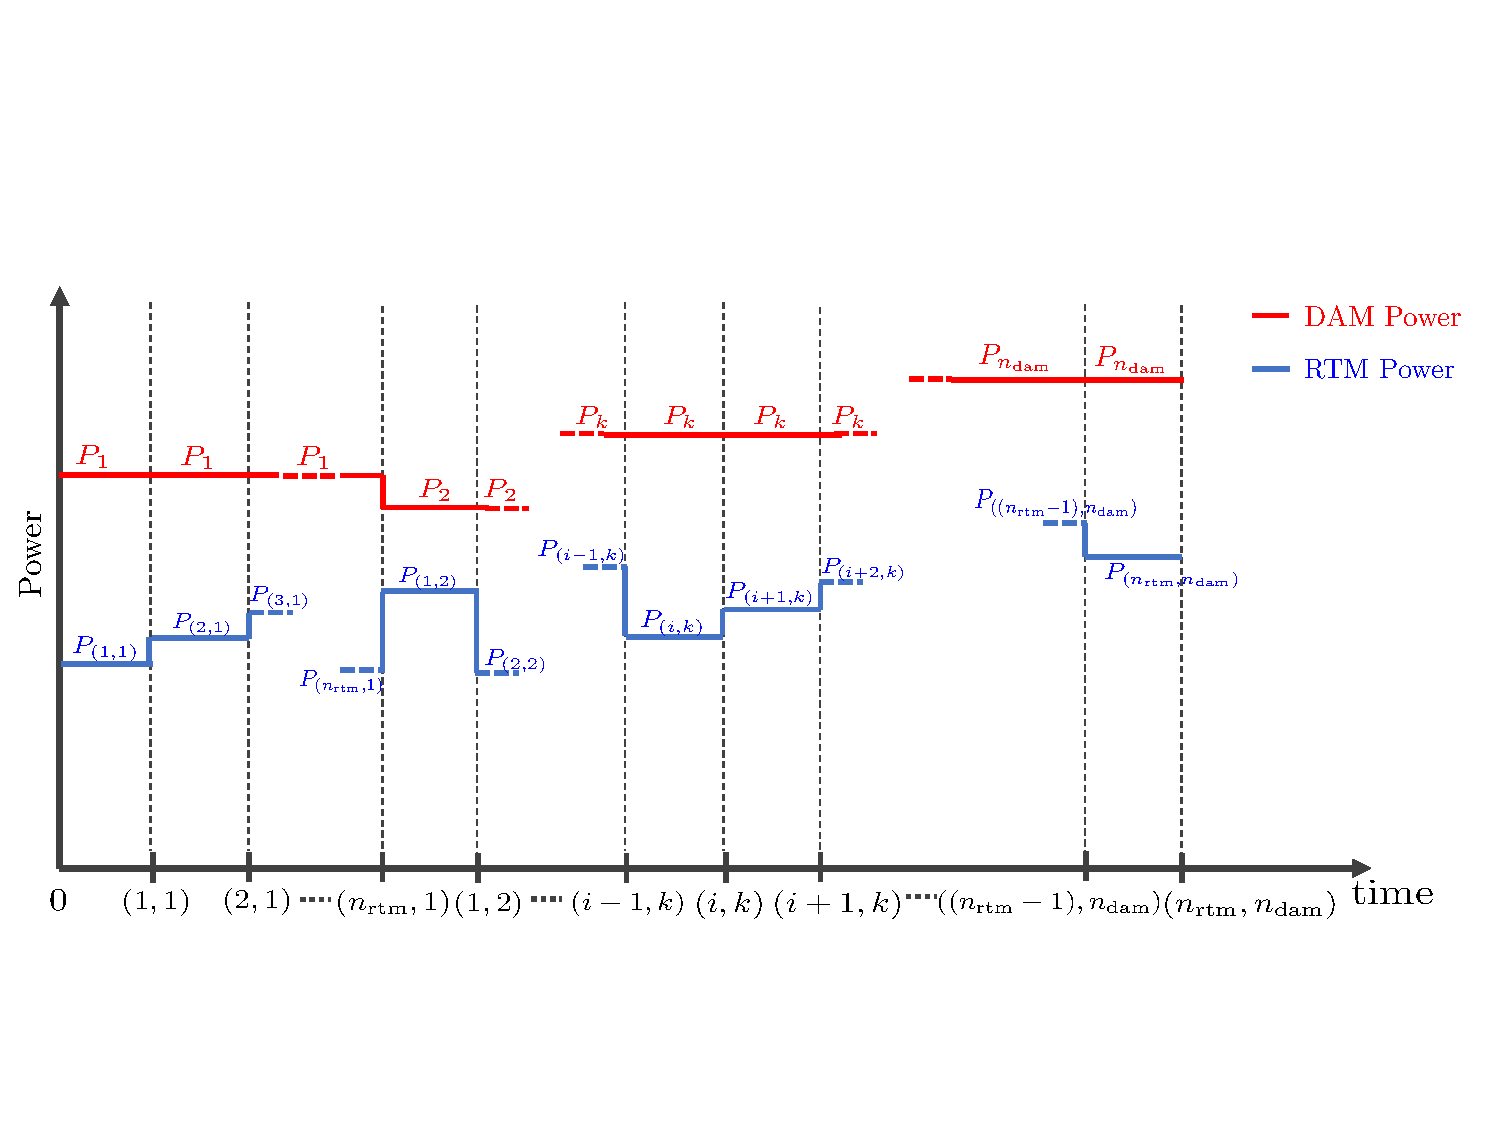
\includegraphics[scale=0.5]{Figures/discretization1.pdf} \caption{Time Discretization and Zero-Order Hold for Variables}\label{fig:discretization}\end{center}
\end{figure}
\FloatBarrier

\subsubsection{Parameters in the model}
\begin{itemize}
\item\textbf{Market parameters:}
\begin{itemize}
\item[\textbullet] $\pi_{k}, \forall k \in \mathcal{T_D}$: Electricity price in day-ahead market in the interval between hour $k-1$ to $k$
\item[\textbullet] $\pi_{i,k}, \forall i \in \mathcal{T_R}, k \in \mathcal{T_D}$: Electricity price in real-time market in the 5-minute interval between $(i-1,k)$ and $(i,k)$ within $k^\text{th}$ hour
\item[\textbullet] $\Delta t$: Time interval (in unit of hours) in the real-time market (which is 5 minutes)
\end{itemize}
\item\textbf{Battery parameters:}
\begin{itemize}
\item[\textbullet] $E_{max} = 0.5$ MWh: Energy storage capacity of the battery
\item[\textbullet] $P_{max} = 0.5$ MW: Maximum discharging or charging rate of the battery
\item[\textbullet] $E_{0} = E_{max}$: Energy stored in the battery before beginning of market participation
\end{itemize}
\item\textbf{Building loads:}
\begin{itemize}
\item[\textbullet] $L_{i,k}, \forall i \in \mathcal{T_R}, k \in \mathcal{T_D}$: Building loads in the 5-minute interval between $(i-1,k)$ and $(i,k)$ within $k^\text{th}$ hour
\end{itemize}
\end{itemize}
\subsubsection{Variables in the model:}
\begin{itemize}
\item \textbf{Decision variables:}
\begin{itemize}
\item[\textbullet] $P_{k}, \forall k \in \mathcal{T_D}$: Power committed by battery in day-ahead market in the interval between hour $k-1$ to $k$
\item[\textbullet] $P_{i,k}, \forall i \in \mathcal{T_R}, k \in \mathcal{T_D}$: Power committed by battery in real-time market in the 5-minute interval between $(i-1,k)$ and $(i,k)$ within $k^\text{th}$ hour
\item[\textbullet] $L^{sup}_{i,k}, \forall i \in \mathcal{T_R}, k \in \mathcal{T_D}$: Power supplied by battery to the building in the 5-minute interval between $(i-1,k)$ and $(i,k)$ within $k^\text{th}$ hour 
\end{itemize}
\item \textbf{State variables:}
\begin{itemize}
\item[\textbullet] $E_{i,k}, \forall i \in \mathcal{T_R}, k \in \mathcal{T_D}$: Energy stored in the battery at time $(i,k)$ (at the end of $i^{th}$ 5-minute interval within $k^\text{th}$ hour) 
\end{itemize}
\end{itemize}
\begin{figure}[h!]
\begin{center}
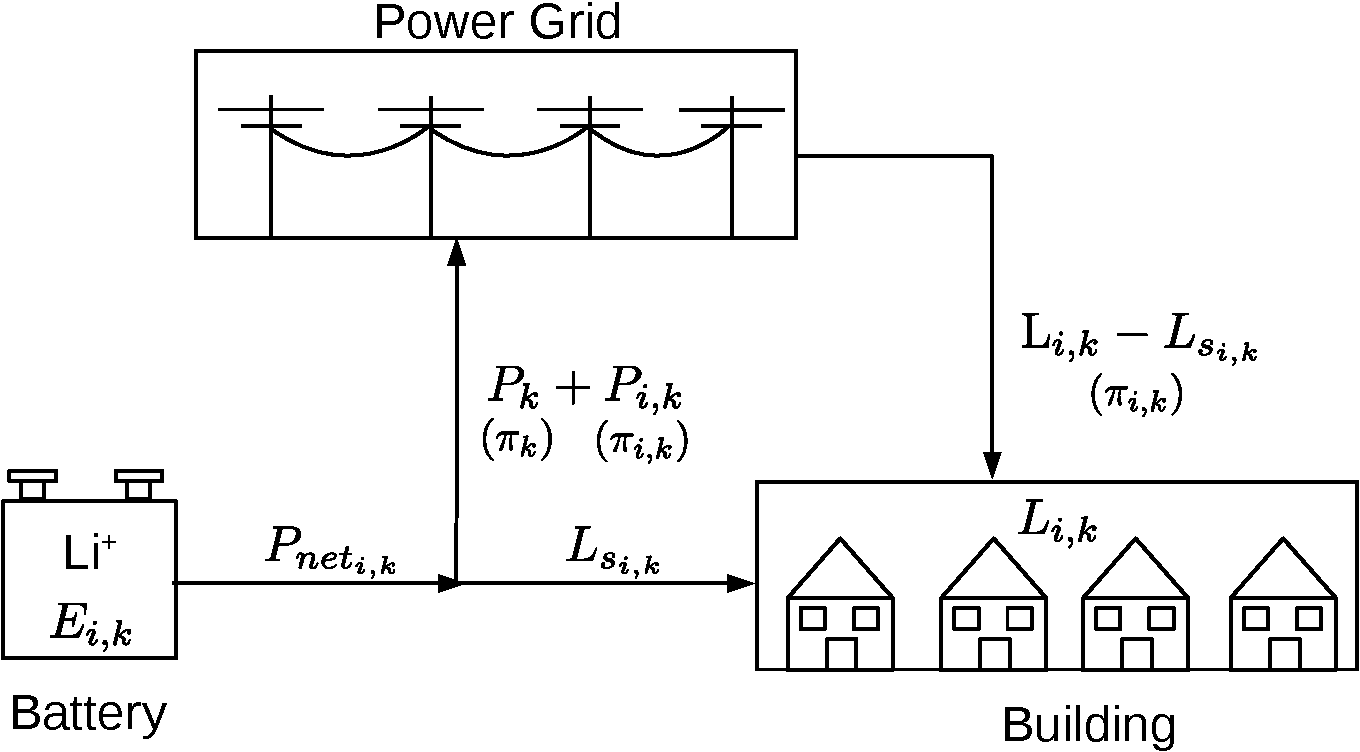
\includegraphics[scale=0.5]{Figures/system_blocks-crop.pdf} \caption{Illustration of Battery-Building System Interconnected with Power Grid}\label{fig:system}\end{center}
\end{figure}
\FloatBarrier
\subsubsection{Constraints and objective function}\label{subsec:const_obj}
\begin{itemize}
\item Net discharge (power) from the battery at any time has to be less than the maximum discharge capacity of the battery, $P_{max}$.
\begin{align}\label{eq:Pnet}
&P_{{net}_{i,k}} = P_{k} + P_{i,k} + L^{sup}_{i,k}, \quad \forall i \in \mathcal{T_R}, k \in \mathcal{T_D}
\end{align}
\item Balance on the energy stored in the battery at each time
\begin{align}\label{eq:ebalance}
E_{i,k} =& E_{i-1,k}- P_{{net}_{i,k}}\Delta t, \quad \forall i \in \mathcal{T_R}, k \in \mathcal{T_D}
\end{align}
In Equation \eqref{eq:ebalance}, $E_{0,k} = E_{0}$ for $k \in \lbrace1\rbrace$ and $E_{0,k} = E_{n_{rtm},k-1}$ for $k \in \mathcal{T_R}\setminus{\lbrace1\rbrace}$. 
\item Bounds on variables:
\begin{subequations}\label{eq:bounds}
\begin{align}
0 & \leq E_{i,j,k} \leq E_{max}, \forall i \in \mathcal{T_R}, k \in \mathcal{T_D}\\
-P_{max} & \leq P_{i,k} \leq P_{max}, \forall i \in \mathcal{T_R}, k \in \mathcal{T_D}\\
-P_{max} & \leq P_{k}\phantom{i,} \leq P_{max}, \forall k \in \mathcal{T_D}\\
-P_{max} & \leq P_{{net}_{i,k}} \leq P_{max}, \forall i \in \mathcal{T_R}, k \in \mathcal{T_D}\\
0 & \leq L^{sup}_{i,k} \leq L_{i,k}, \forall i \in \mathcal{T_R}, k \in \mathcal{T_D}
\end{align}
\end{subequations}
\item Objective Function:
\begin{align}\label{objective}
\min \quad -\sum\limits_{i \in \mathcal{T_R}}\sum\limits_{k \in \mathcal{T_R}} \pi_{i,k}P_{i,k}\Delta t - \sum\limits_{k \in \mathcal{T_D}}\pi_{k}P_{k}\Delta t n_{rtm} + \sum\limits_{i \in \mathcal{T_R}}\sum\limits_{k \in \mathcal{T_R}} \pi_{i,k}(L_{i,k}-L^{sup}_{i,k})\Delta t
\end{align}
\end{itemize}

\subsection{Optimization Model Under Uncertainty} \label{subsec:opt_unc}
Now, we consider uncertainty in the building loads and extend the optimization formulation in deterministic setting (Section \ref{subsec:deterministic}) to formulate an extensive form of stochastic optimization problem to minimize the expected cost (or maximize expected revenue) for the building-battery system. In the formulation for the optimization problem under uncertainty, we consider all the market participating conditions to be the same as in the deterministic setting except for the uncertainty in the loads. We use the same sets of time indices, time-discretization approach and variable/parameter notations as developed in Section \ref{subsec:deterministic} with the exception that uncertainty has to be added to all real-time variables because of the uncertain loads. We represent this uncertainty with a sample space $\Xi$ and an outcome from this space is denoted by $\xi$. As described in Section \ref{sec:setting}, we consider that when a scenario $\xi \in \Xi$ realizes at an hour $k$ the loads at all real-time subintervals between hour $k-1$ and $k$ become known and the scenario-tree grows at every hour. So, the uncertain load at every time is denoted as $L_{i,k}(\xi)$. Similarly, we denote the resulting uncertainty in all real-time variables, namely the energy transacted by the battery with real-time market ($P_{i,k}(\xi)$), the energy supplied by the battery to the building ($L^{sup}_{i,k}(\xi)$) and the energy stored in the battery at every time ($E_{i,k}(\xi)$). The day-ahead energy participation by the battery is a first-stage decision which needs to be made before the realization of uncertainty. Furthermore, for the extensive form of the stochastic programming model, we assume that the uncertainty can be represented by a set $\mathcal{S}$ of $N$ possible scenarios and all possible realizations of uncertainty lie in this set. So, $s \in \mathcal{S}$ represents a possible scenario of the realization of uncertainty. Also, we make the assumption that the scenarios are equiprobable. We use these assumptions to build the extensive form of the stochastic program to minimize the expected cost (maximize expected revenue) for the system and is described below.

\subsubsection{Variables in the extensive form model}\label{subsubsec:var_ext}
\begin{itemize}
\item \textbf{Decision variables:}
\begin{itemize}
\item[\textbullet] $P_{k,s}, \forall k \in \mathcal{T_D}, \forall s \in \mathcal{S}$: Power committed by battery in day-ahead market in the interval between hour $k-1$ to $k$ in scenario $s$
\item[\textbullet] $P_{i,k,s}, \forall i \in \mathcal{T_R}, k \in \mathcal{T_D}, \forall s \in \mathcal{S}$: Power committed by battery in real-time market in the 5-minute interval between $(i-1,k)$ and $(i,k)$ within $k^\text{th}$ hour in scenario $s$
\item[\textbullet] $L^{sup}_{i,k,s}, \forall i \in \mathcal{T_R}, k \in \mathcal{T_D}, \forall s \in \mathcal{S}$: Power supplied by battery to the building in the 5-minute interval between $(i-1,k)$ and $(i,k)$ within $k^\text{th}$ hour in scenario $s$
\end{itemize}
\item \textbf{State variables:}
\begin{itemize}
\item[\textbullet] $E_{i,k,s}, \forall i \in \mathcal{T_R}, k \in \mathcal{T_D}, \forall s \in \mathcal{S}$: Energy stored in the battery at time $(i,k)$ (at the end of $i^{th}$ 5-minute interval within $k^\text{th}$ hour) in scenario $s$
\end{itemize}
\end{itemize}

\subsubsection{Constraints and objective function}\label{subsubsec:const_obj_ext}
\begin{itemize}
\item Net discharge (power) from the battery at any time has to be less than the maximum discharge capacity of the battery, $P_{max}$.
\begin{align}\label{eq:Pnet_unc}
&P_{{net}_{i,k,s}} = P_{k,s} + P_{i,k,s} + L^{sup}_{i,k,s}, \quad \forall i \in \mathcal{T_R}, k \in \mathcal{T_D}, s \in \mathcal{S}
\end{align}
\item Balance on the energy stored in the battery at each time
\begin{align}\label{eq:ebalance_unc}
E_{i,k,s} =& E_{i-1,k,s}- P_{{net}_{i,k,s}}\Delta t, \quad \forall i \in \mathcal{T_R}, k \in \mathcal{T_D}, s \in \mathcal{S}
\end{align}
In equation \eqref{eq:ebalance_unc}, $E_{0,k,s} = E_{0}$ for $k \in \lbrace1\rbrace$ and $E_{0,k,s} = E_{n_{rtm},k-1,s}$ for $k \in \mathcal{T_R}\setminus{\lbrace1\rbrace}, s \in \mathcal{S}$. 
\item Bounds on variables:
\begin{subequations}\label{eq:bounds_unc}
\begin{align}
0 & \leq E_{i,j,k,s} \leq E_{max}, \forall i \in \mathcal{T_R}, k \in \mathcal{T_D}\\
-P_{max} & \leq P_{i,k,s} \leq P_{max}, \forall i \in \mathcal{T_R}, k \in \mathcal{T_D}, s \in \mathcal{S}\\
-P_{max} & \leq P_{k,s}\phantom{i,} \leq P_{max}, \forall k \in \mathcal{T_D}, s \in \mathcal{S}\\
-P_{max} & \leq P_{{net}_{i,k,s}} \leq P_{max}, \forall i \in \mathcal{T_R}, k \in \mathcal{T_D}, s \in \mathcal{S}\\
0 & \leq L^{sup}_{i,k,s} \leq L_{i,k,s}, \forall i \in \mathcal{T_R}, k \in \mathcal{T_D}, s \in \mathcal{S}
\end{align}
\end{subequations}
\item Nonanticipativity constraints for first-stage decisions ($P_{k,s}$):
\begin{align}\label{eq:nonant_unc}
P_{k,s} =& \frac{1}{N} \sum\limits_{s \in \mathcal{S}} P_{k,s}, \quad \forall k \in \mathcal{T_D}, s \in \mathcal{S}
\end{align}
\item Objective Function:
\begin{align}\label{objective_unc}
\min \quad \frac{1}{N} \sum\limits_{s \in \mathcal{S}} \left[-\sum\limits_{i \in \mathcal{T_R}}\sum\limits_{k \in \mathcal{T_R}} \pi_{i,k}P_{i,k,s}\Delta t - \sum\limits_{k \in \mathcal{T_D}}\pi_{k}P_{k,s}\Delta t n_{rtm} + \sum\limits_{i \in \mathcal{T_R}}\sum\limits_{k \in \mathcal{T_R}} \pi_{i,k}(L_{i,k,s}-L^{sup}_{i,k,s})\Delta t \right]
\end{align}
\end{itemize}

\section{Computational Experiments}\label{sec:exp}
\subsection{Studies with Two-Stage Approximations}
If we consider all the paths in the scenario tree over 168 stages (1-week planning period) taking 50 realizations of load profile at every stage, the total number of possible scenarios is $50^{168}$. The problem size for the full scenario tree is huge which will take an enormous amount of time and will not be practically useful for the decision-maker. 

To tackle this difficulty of the huge size of the stochastic program, we use the two-stage approximation for a multi-stage problem. We also use sample average approximation to limit the number of scenarios. In this approach, we sample a finite number of random paths (realizations of load profiles over 168 hours) along the scenario tree and obtain the expected revenue from operating the battery in the setting described in \ref{subsec:opt_unc}. We also obtain a confidence interval over the expected revenue by repeating the same process many times (taking multiple batches of sampled paths).

We use this approach to study the economic potential of electricity markets and to estimate bounds on the expected revenue obtained by participating in the markets.

\subsubsection{Economic Potential of Different Timescales of Electricity Markets}\label{subsec:economic}
In this case study, we sample 50 scenario paths (out of the $50^{168}$ possibilities) for a week's time period. We then construct a full model for for this week and use real price signals from 01/01/2015 to 01/07/2015 in California ISO \footnote{http://oasis.caiso.com/mrioasis/logon.do}. For every 1 hour interval in the model, we sample a scenario, and use the load data corresponding to that scenario for the 12 intervals (5 minutes each) in that hour. This helps to reduce the size of scenario tree (from $50^{168 \times 12}$ to $50^{168}$). We solve this model (with 50 sampled paths) 100 times to get a confidence interval on the expected revenue. We then compare this expected revenue (obtained by participating in both real-time and day-ahead market) to the cases when the battery participates only in either real-time or day-ahead market alone.
\begin{table}[!ht]\centering
\caption{Revenue Breakup from Participation in Different Markets}
\begin{tabular}{|C{3cm}|C{2.5cm}|C{3.5cm}|C{3cm}|C{2.5cm}|} 
\hline 
Market Participated  & Total Revenue (\$) & Unmet Load Cost (\$) & DAM Revenue  (\$) & RTM Revenue (\$) \\
\hline 
DAM + RTM & 711.08 & -8.75 & 793.12 & -90.79 \\ 
\hline 
DAM & -921.73 & 77.00 & -844.73 & N/A \\ 
\hline 
RTM & -31.32 & -9.10 & N/A & -40.42 \\ 
\hline 
None & -10,293.23 & 10,293.23 & N/A & N/A \\ 
\hline 
\end{tabular} \label{tab:rev_comp} 
\end{table}
Highest revenue is earned when the battery participates in both the real-time and day-ahead markets (Table \ref{tab:rev_comp}). Whereas, if it participates in just day-ahead or real-time market alone, the revenue is much less or even negative (results in loss). Consider the case when it participates in only day-ahead market. It is evident from Figure \ref{fig:Pdam_onlydam} and \ref{fig:cumulative_rev_onlydam} that the battery needs to charge itself (buy energy from the grid) in order to meet the building load demands. The price of energy is on average higher in day-ahead market than that in real-time markets. Thus with no participation in real-time market it does not have the flexibility to buy energy from the real-time market at lower prices and sell to day-ahead market (at a higher price) to make profits. The building loads need to be met in real-time (at every 5-minute interval) while the battery has the opportunity to buy or sell energy from the grid only at every hour. Thus the battery is forced to store enough energy to meet the building requirement for an hour by buying energy in hourly intervals from the day-ahead market. Whenever it has slightly excess energy available it tries to sell that energy to the day-ahead market to minimize the overall cost. 
\begin{figure}[h!]
\begin{center}
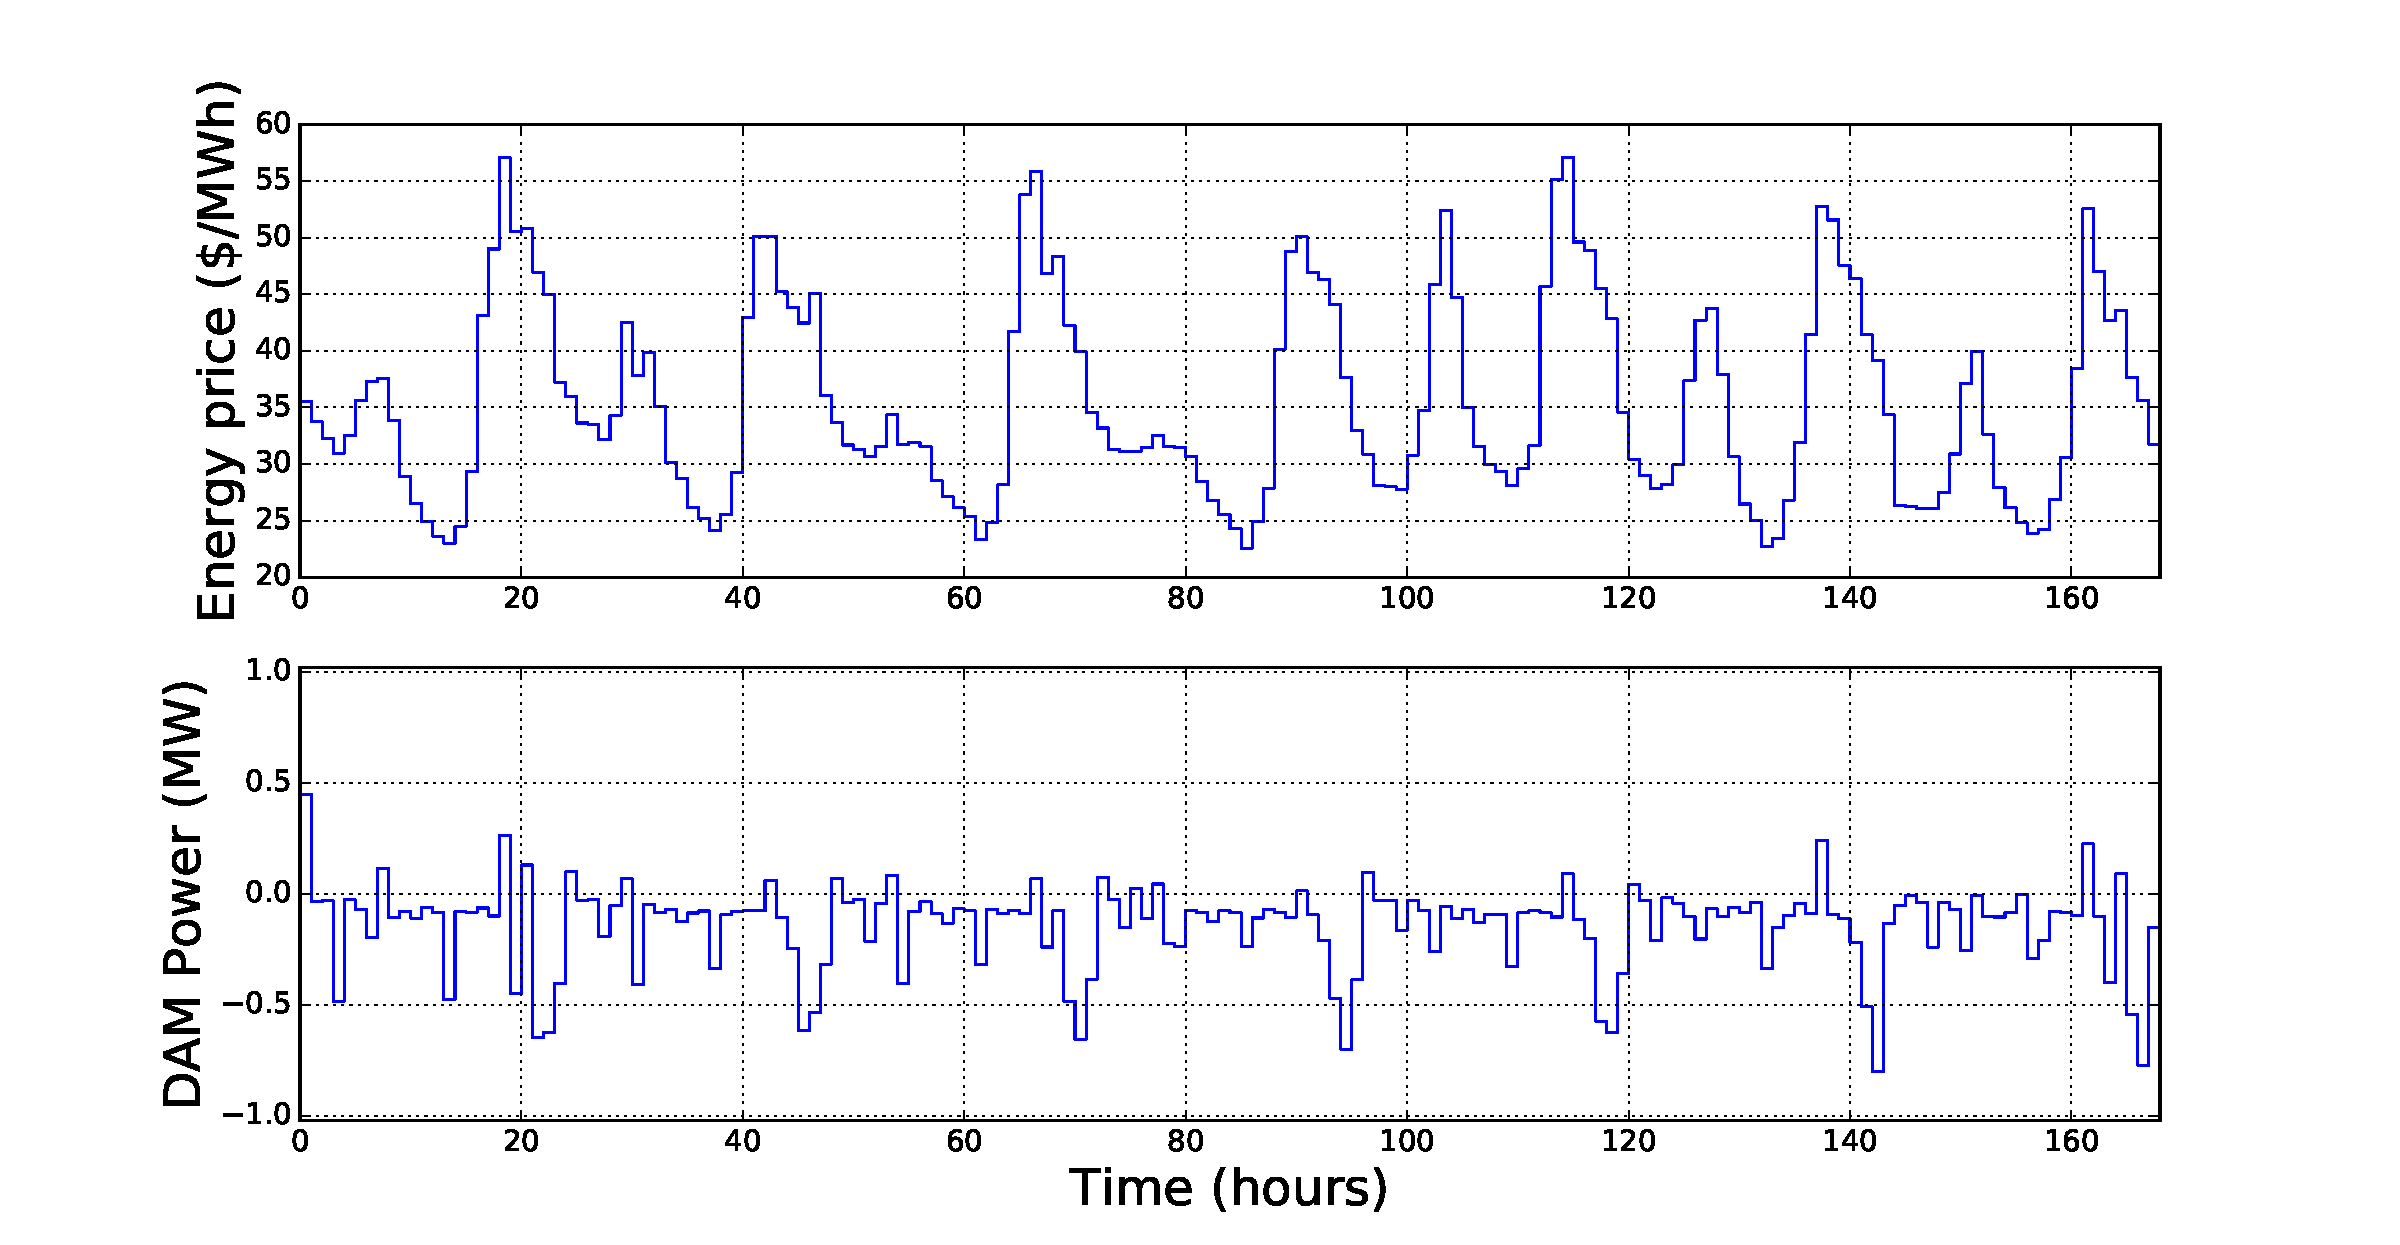
\includegraphics[width=0.7\textwidth]
{Figures/Plots/onlydam/Pdam_fp_st.pdf} \caption{Energy participation policy when battery participates only in day-ahead market.}\label{fig:Pdam_onlydam}\end{center}
\end{figure}
\FloatBarrier
\begin{figure}[h!]
\begin{subfigure}[b]{\textwidth}
\centering
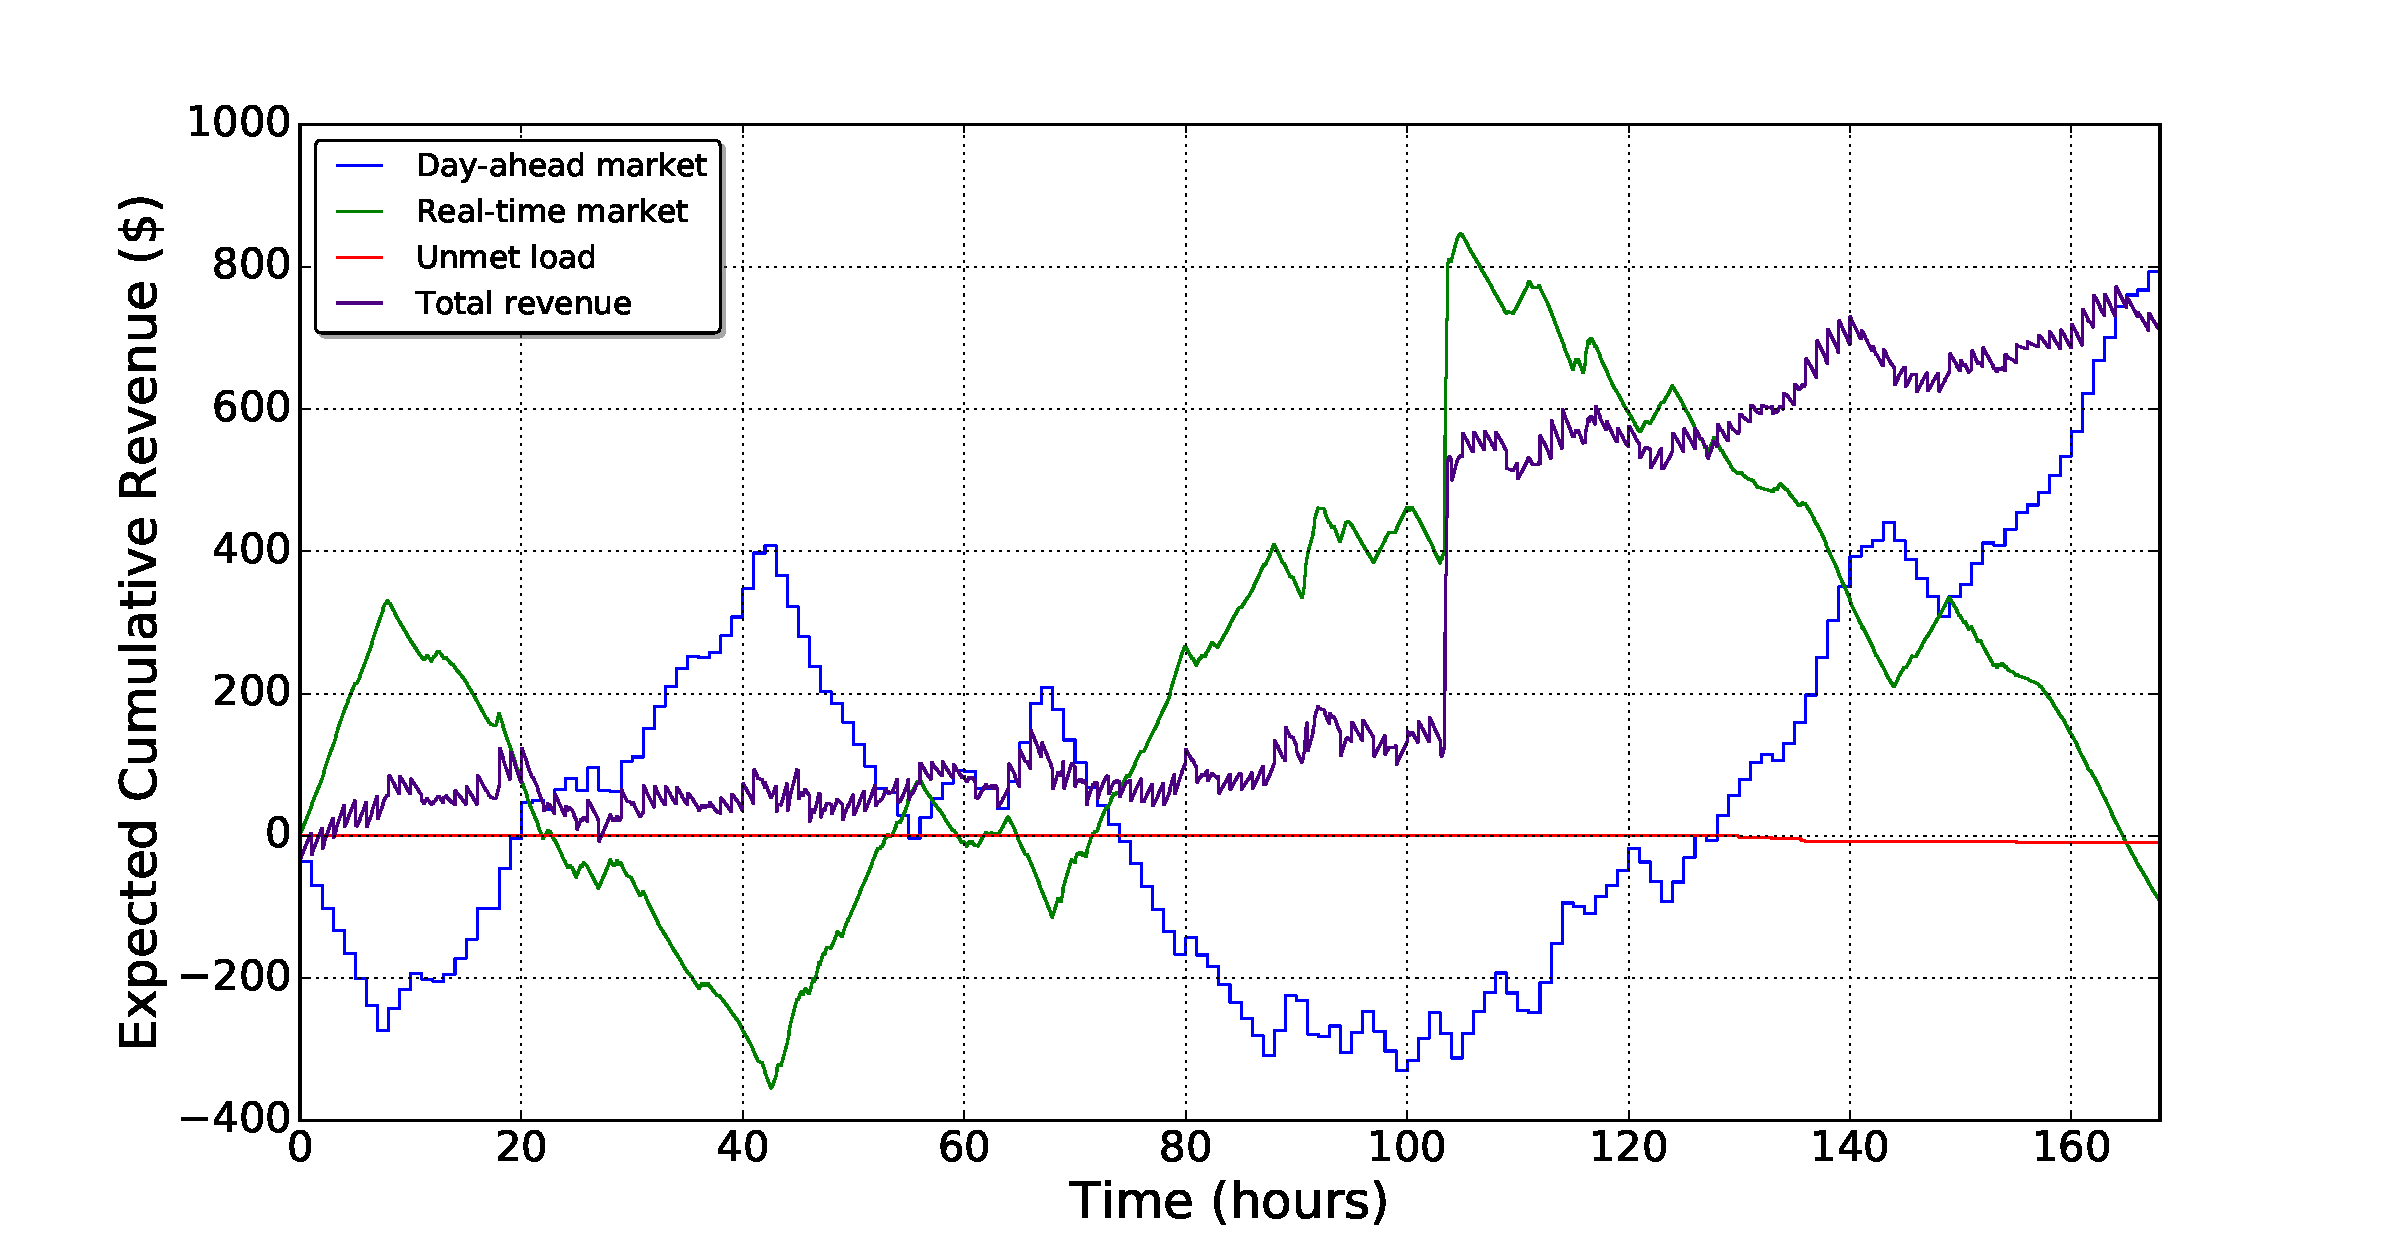
\includegraphics[width=0.7\textwidth]{Figures/Plots/fullproblem_stoch/cumulative_rev_fp_st.pdf} \caption{Participating in both day-ahead and real-time markets}\label{fig:cumulative_rev_fp_st}
\end{subfigure}\hfill
\begin{subfigure}[b]{\textwidth}
\centering
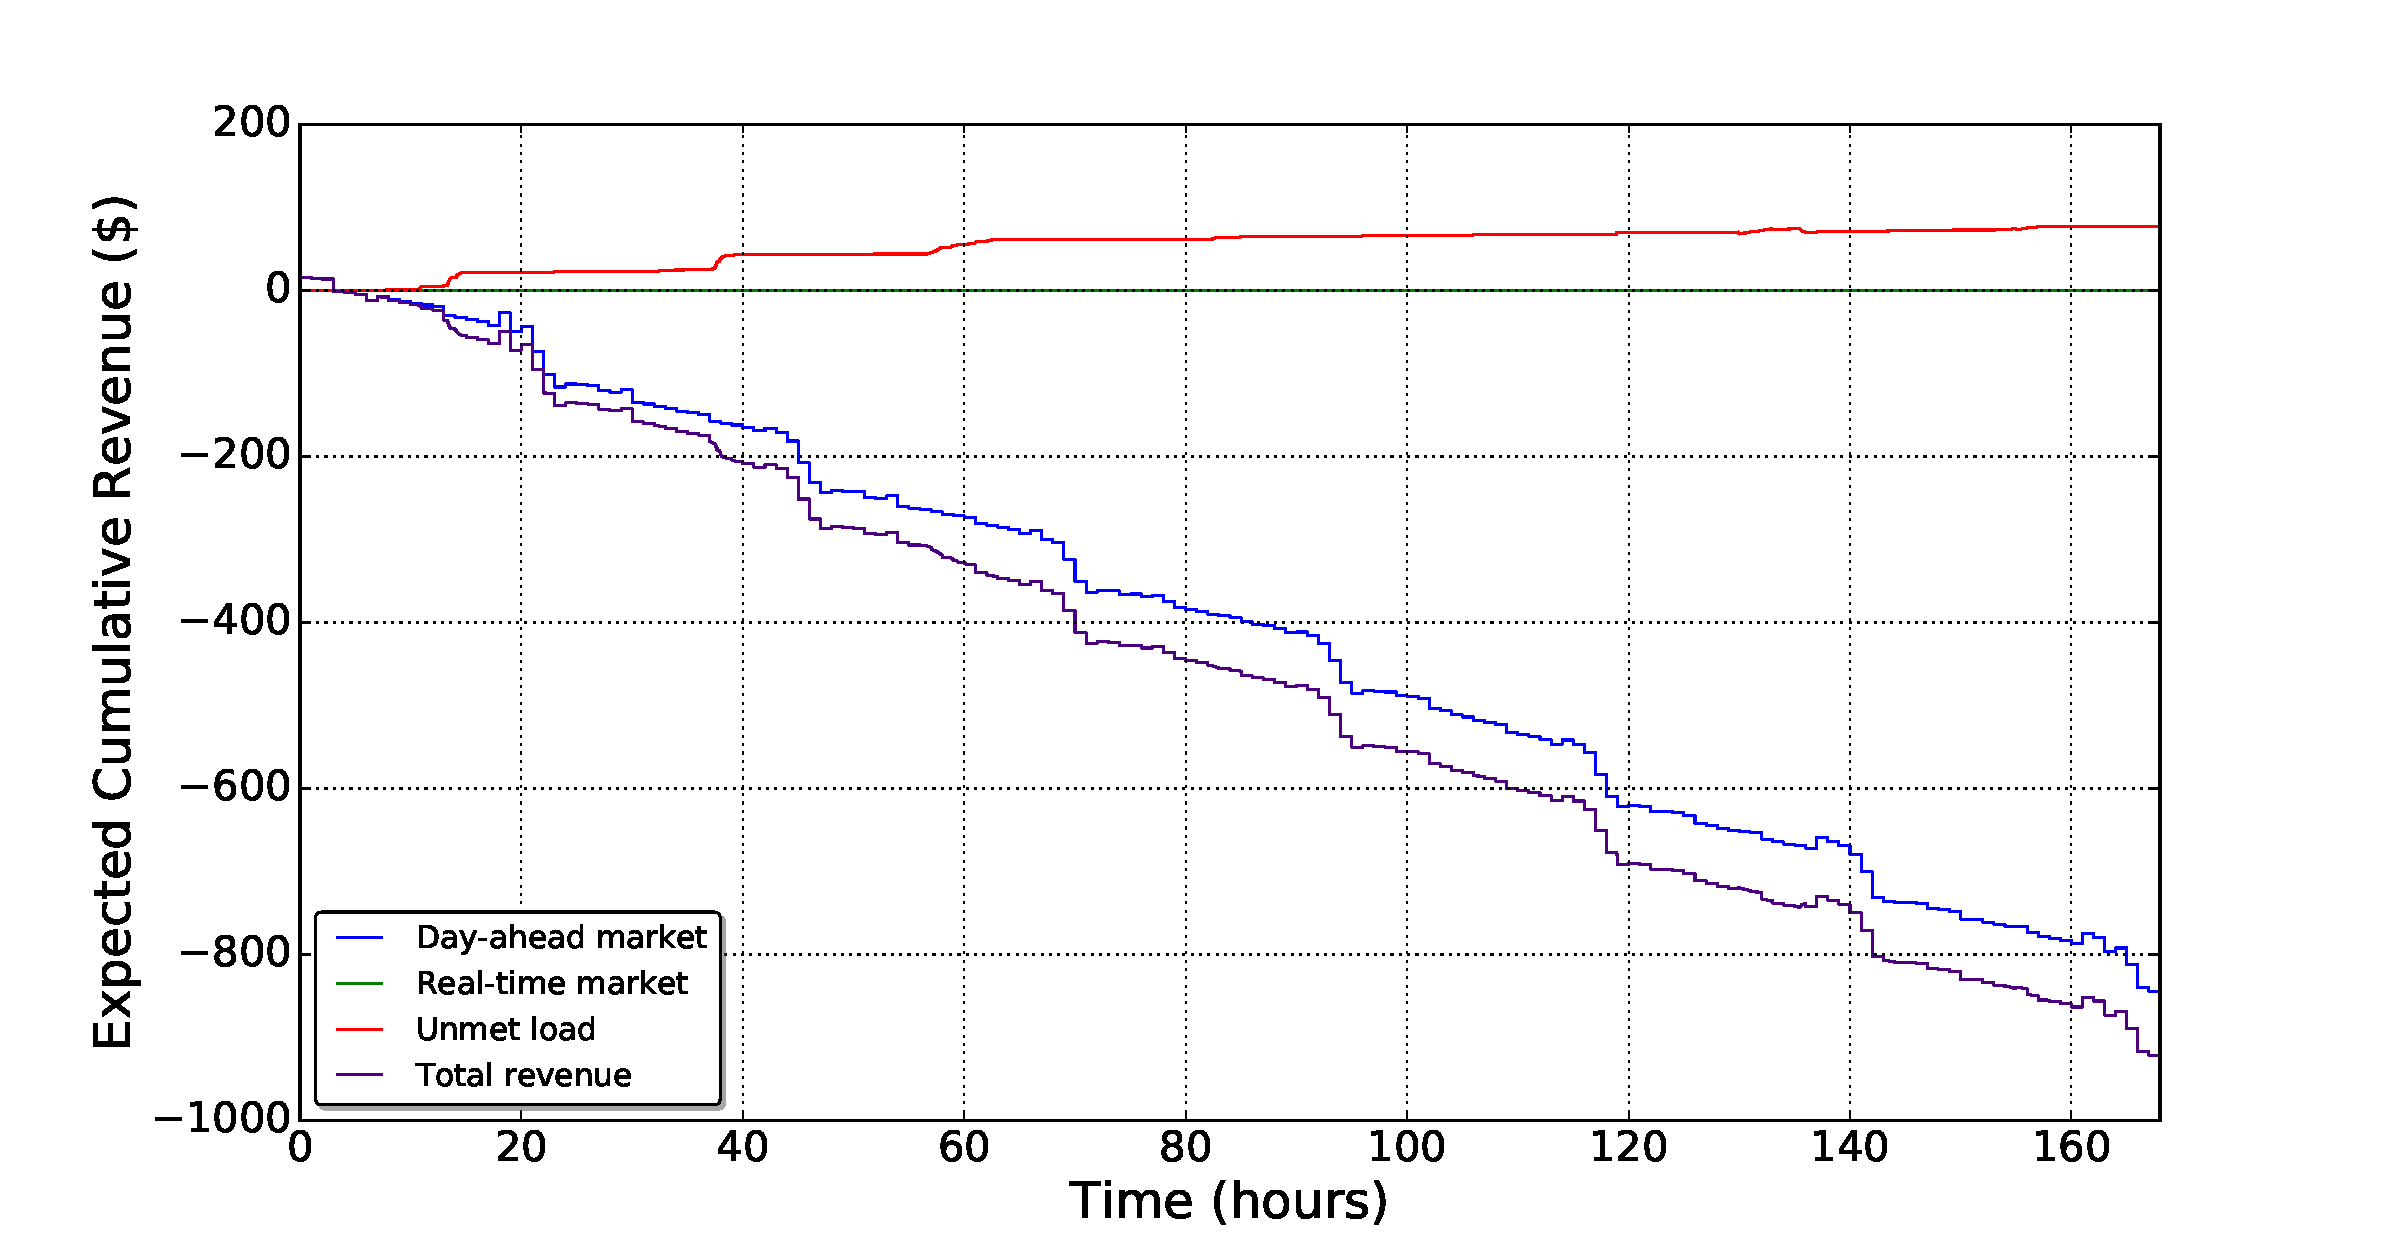
\includegraphics[width=0.7\textwidth]
{Figures/Plots/onlydam/cumulative_rev_fp_st.pdf} \caption{Participating only in day-ahead market}\label{fig:cumulative_rev_onlydam}
\end{subfigure}
\caption{Trajectory of cumulative revenues when battery participates in both RTM and DAM and only DAM alone}
\end{figure}
\FloatBarrier
On the other hand, when it participates in both day-ahead and real-time markets, it has the flexibility to buy from the real-time market and sell to the day-ahead market (Figures \ref{fig:cumulative_rev_fp_st} and \ref{fig:power_both}) while saving sufficient energy to meet the building requirement in real-time. This is possible because the real-time electricity prices are slightly lower than the day-ahead market prices on average. The real-time prices also fall below the day-ahead market prices very often (Figures \ref{fig:Pdam_fp_st} and \ref{fig:Prtm_fp_st}) and because of its fast dynamics, the battery can capture these moments by buying from real-time market and selling in day-ahead market to make profit. 
\begin{figure}[h!]\label{fig:power_both}
\begin{subfigure}{\textwidth}
\centering
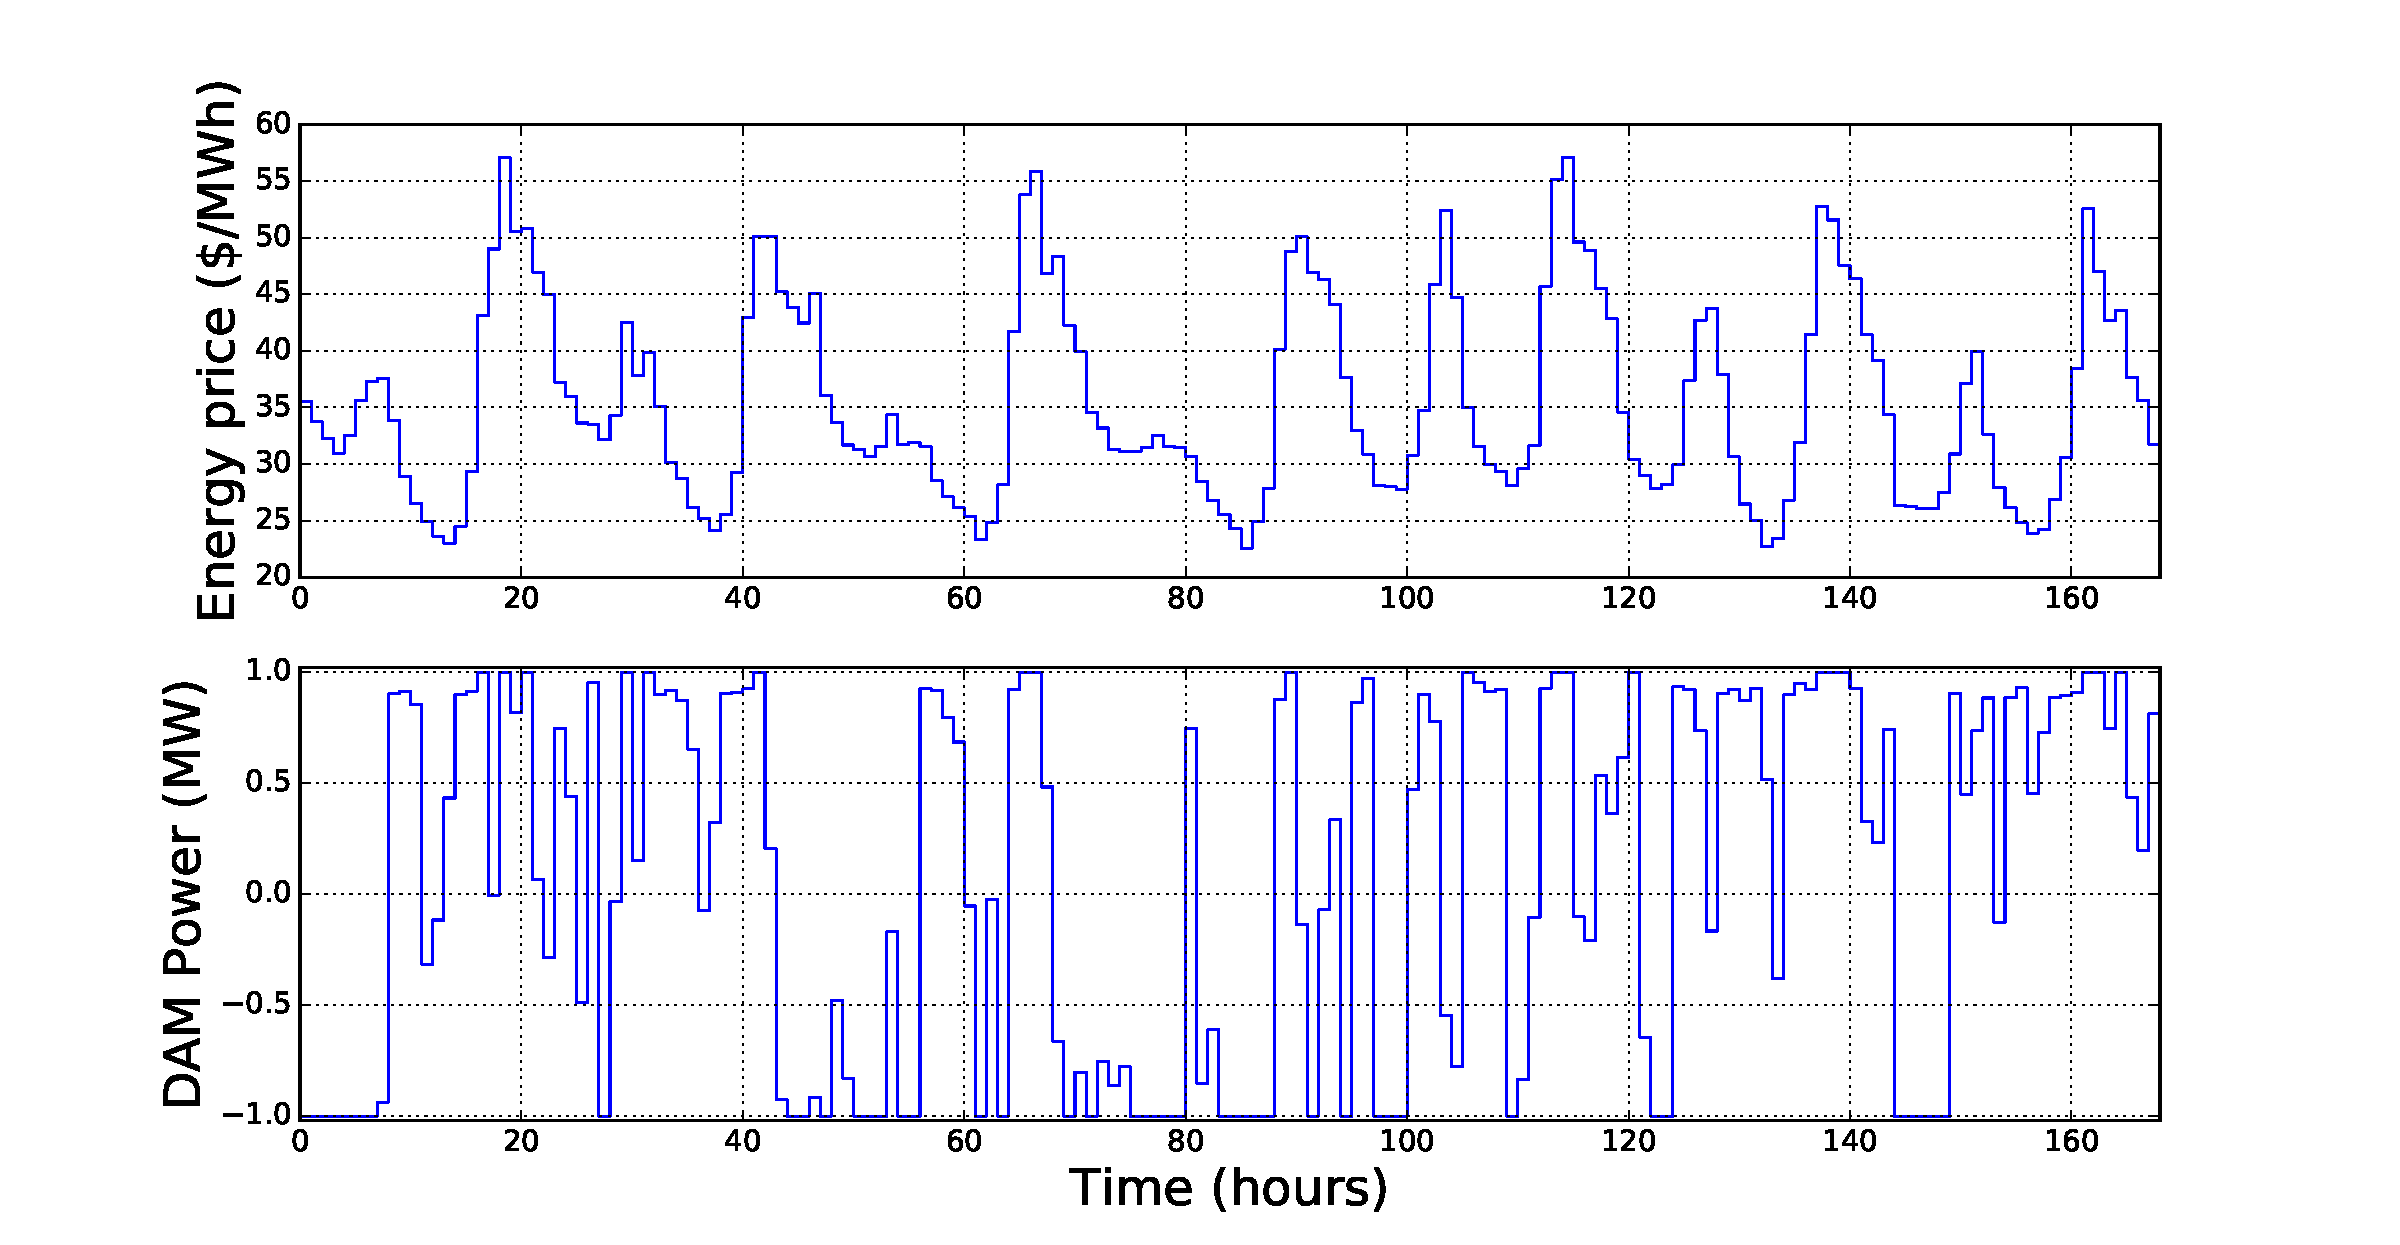
\includegraphics[width=0.6\textwidth]{Figures/Plots/fullproblem_stoch/Pdam_fp_st.pdf} \caption{Day-ahead market}\label{fig:Pdam_fp_st}
\end{subfigure}
\begin{subfigure}{\textwidth}
\centering
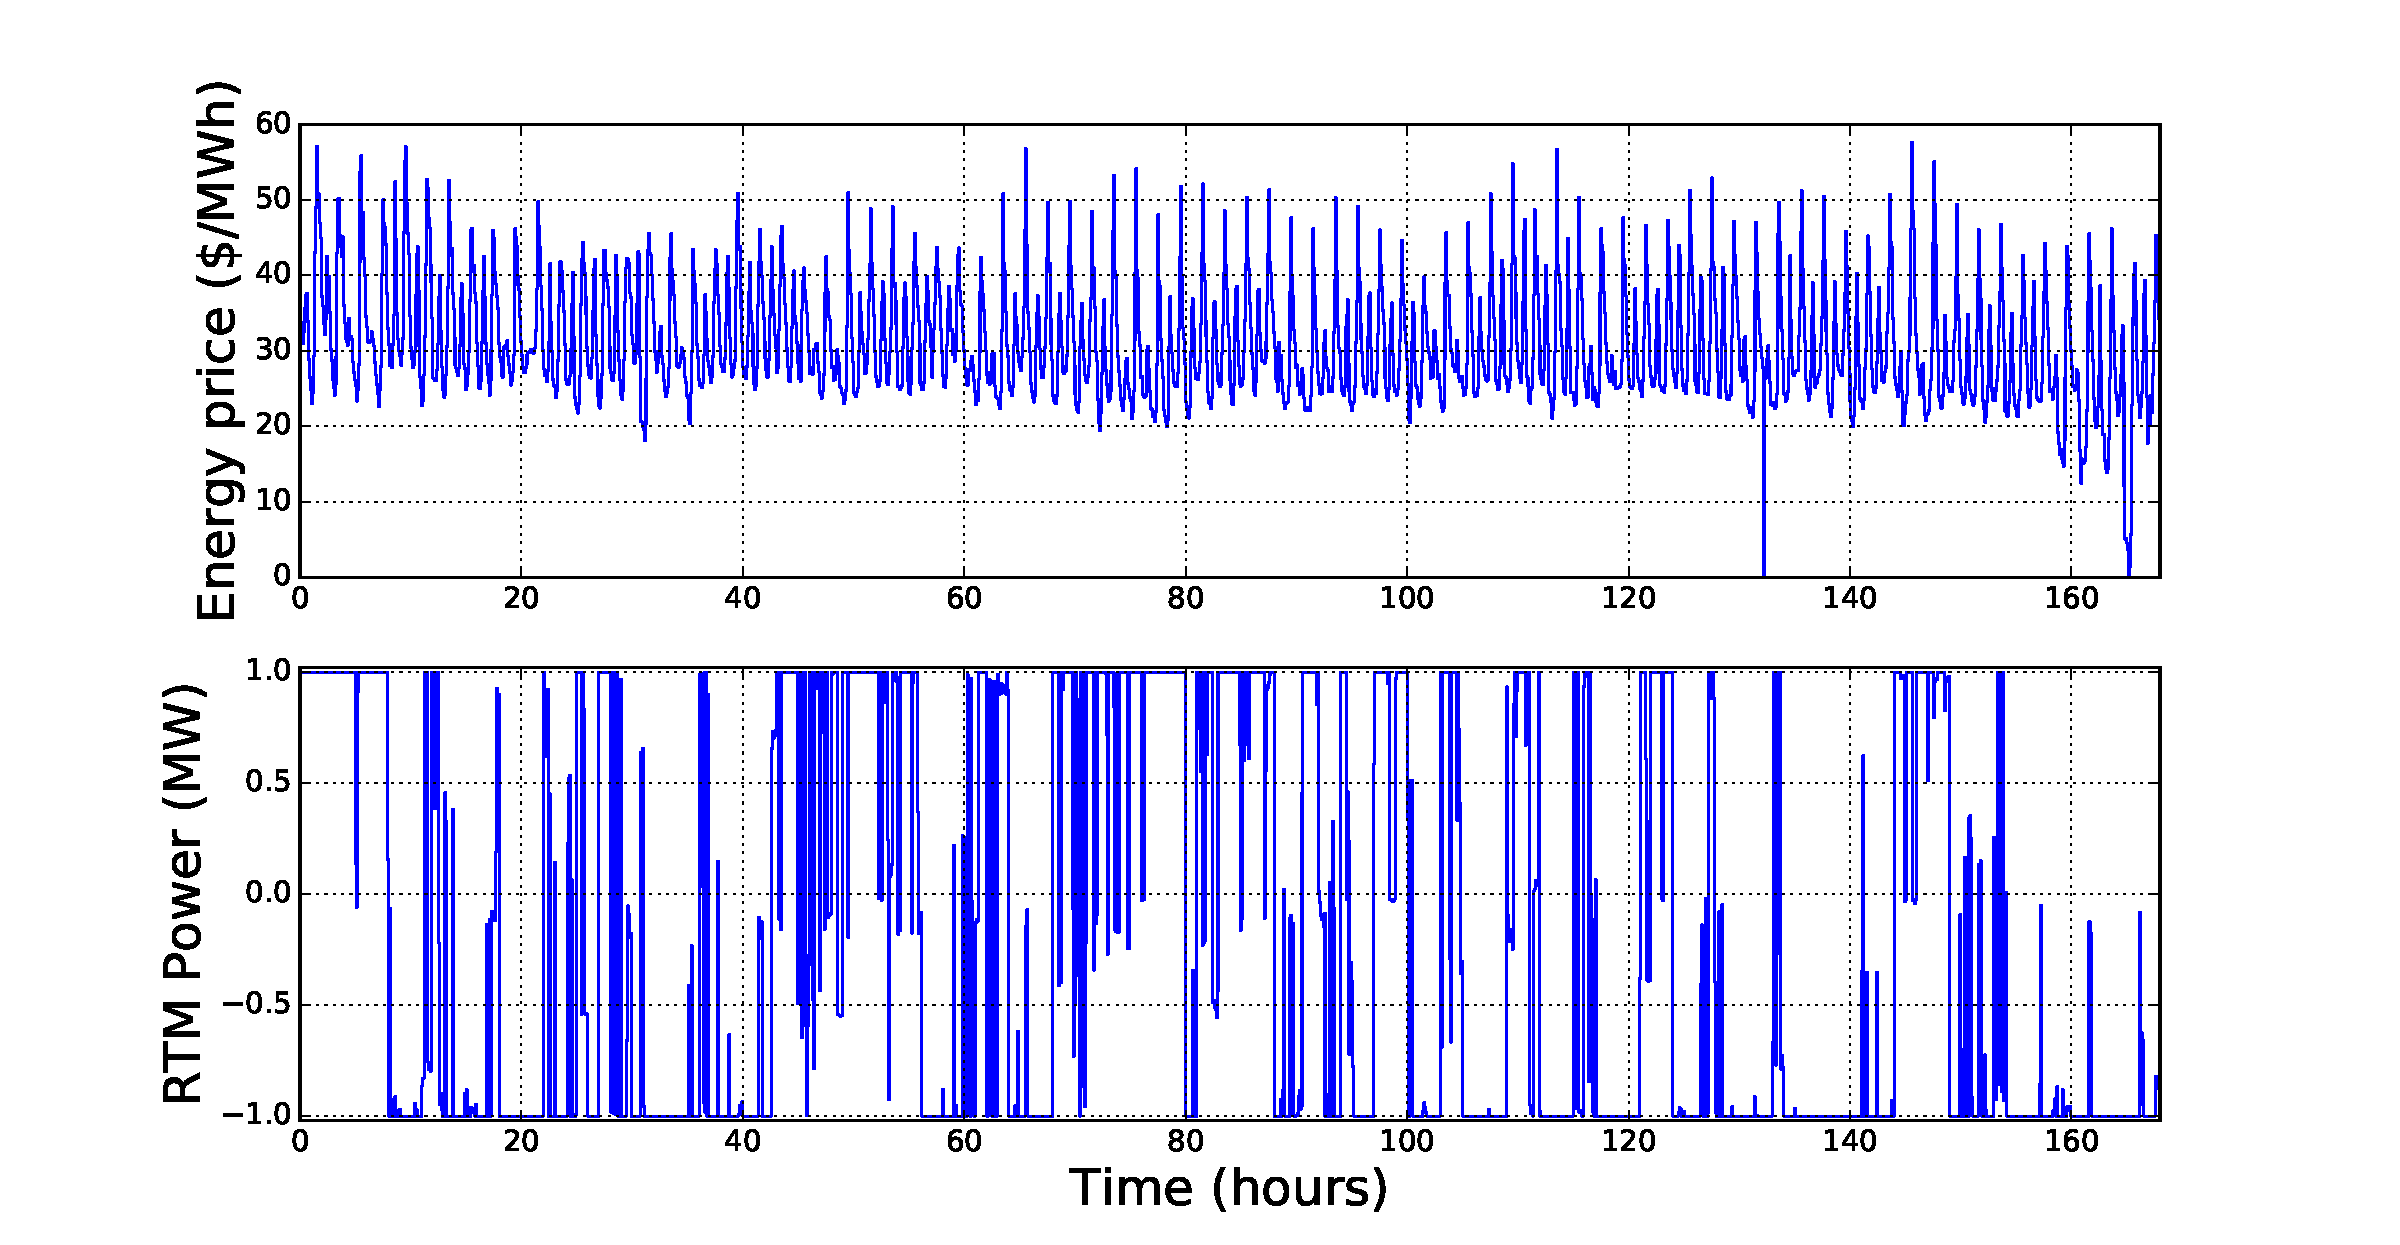
\includegraphics[width=0.6\textwidth]{Figures/Plots/fullproblem_stoch/Prtm_fp_st.pdf} \caption{Real-time market}\label{fig:Prtm_fp_st}
\end{subfigure}
\caption{Energy participation policy when battery participates in both day-ahead and real-time markets}
\end{figure}
\FloatBarrier
Figure \ref{fig:netpower_fp_st} provides the net charge-discharge policy of the battery when it participates in markets at both timescales and Figure \ref{fig:soc_fp_st} depicts how the state of charge of the battery, which is the fraction of energy storage capacity of the battery, changes with time during its participation in the markets. The state of charge of the battery is proportional to the energy level of the battery at any time, so it represents the variation of the state variable in our problem.
\begin{figure}[h!]
\begin{subfigure}{\textwidth}
\centering
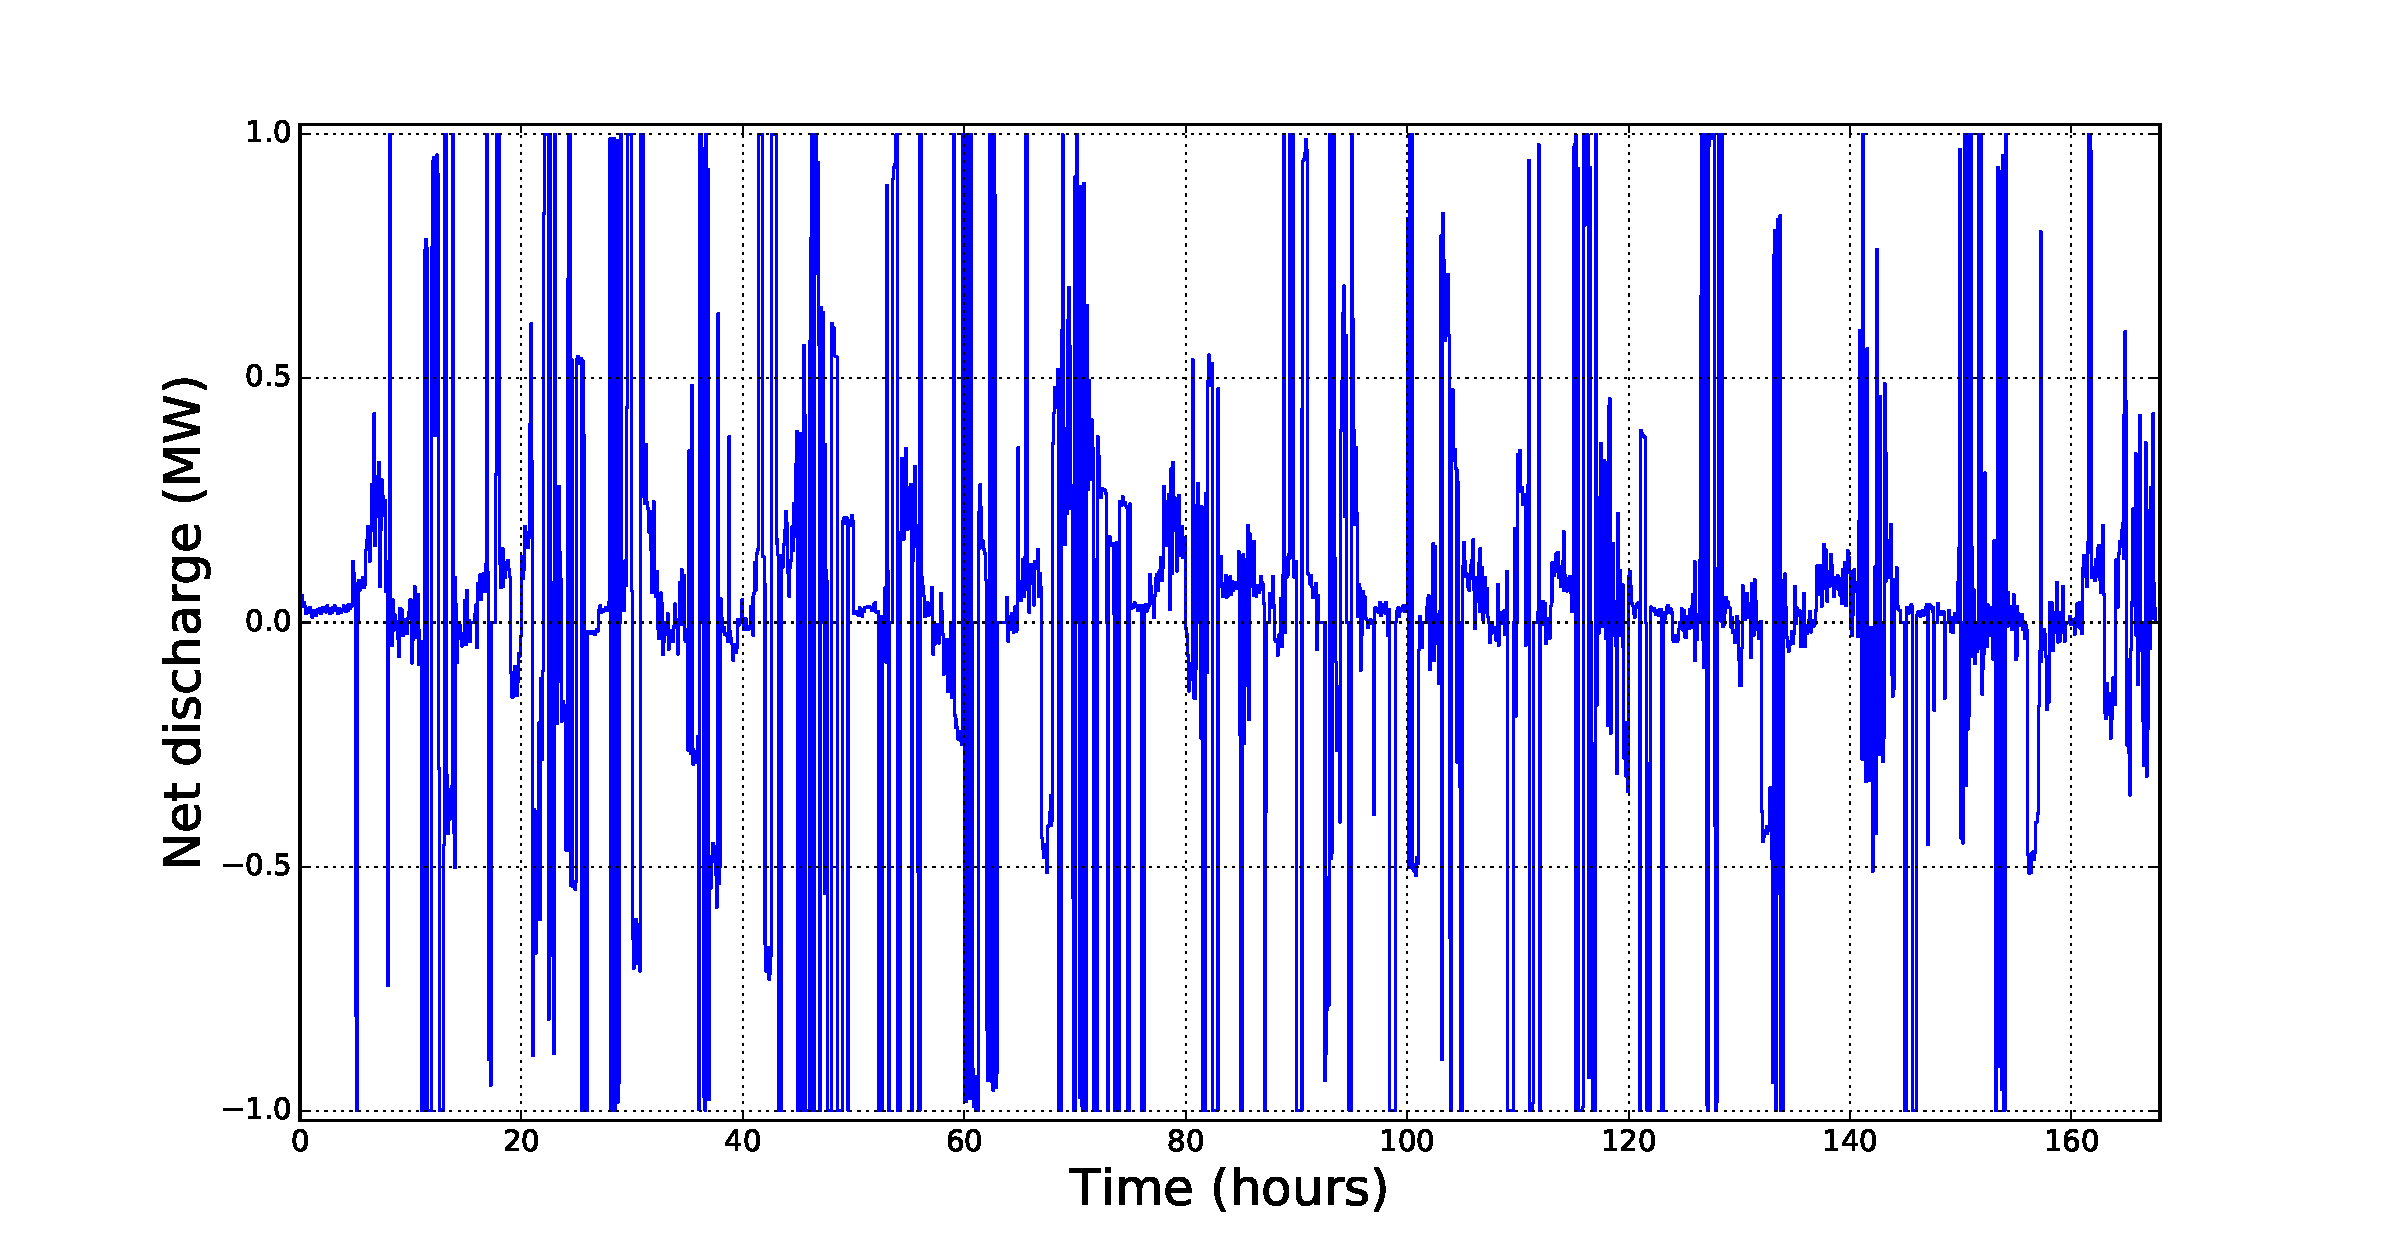
\includegraphics[width=0.7\textwidth]{Figures/Plots/fullproblem_stoch/netpower_fp_st.pdf} \caption{Net battery discharge}\label{fig:netpower_fp_st}
\end{subfigure}
\begin{subfigure}{\textwidth}
\centering
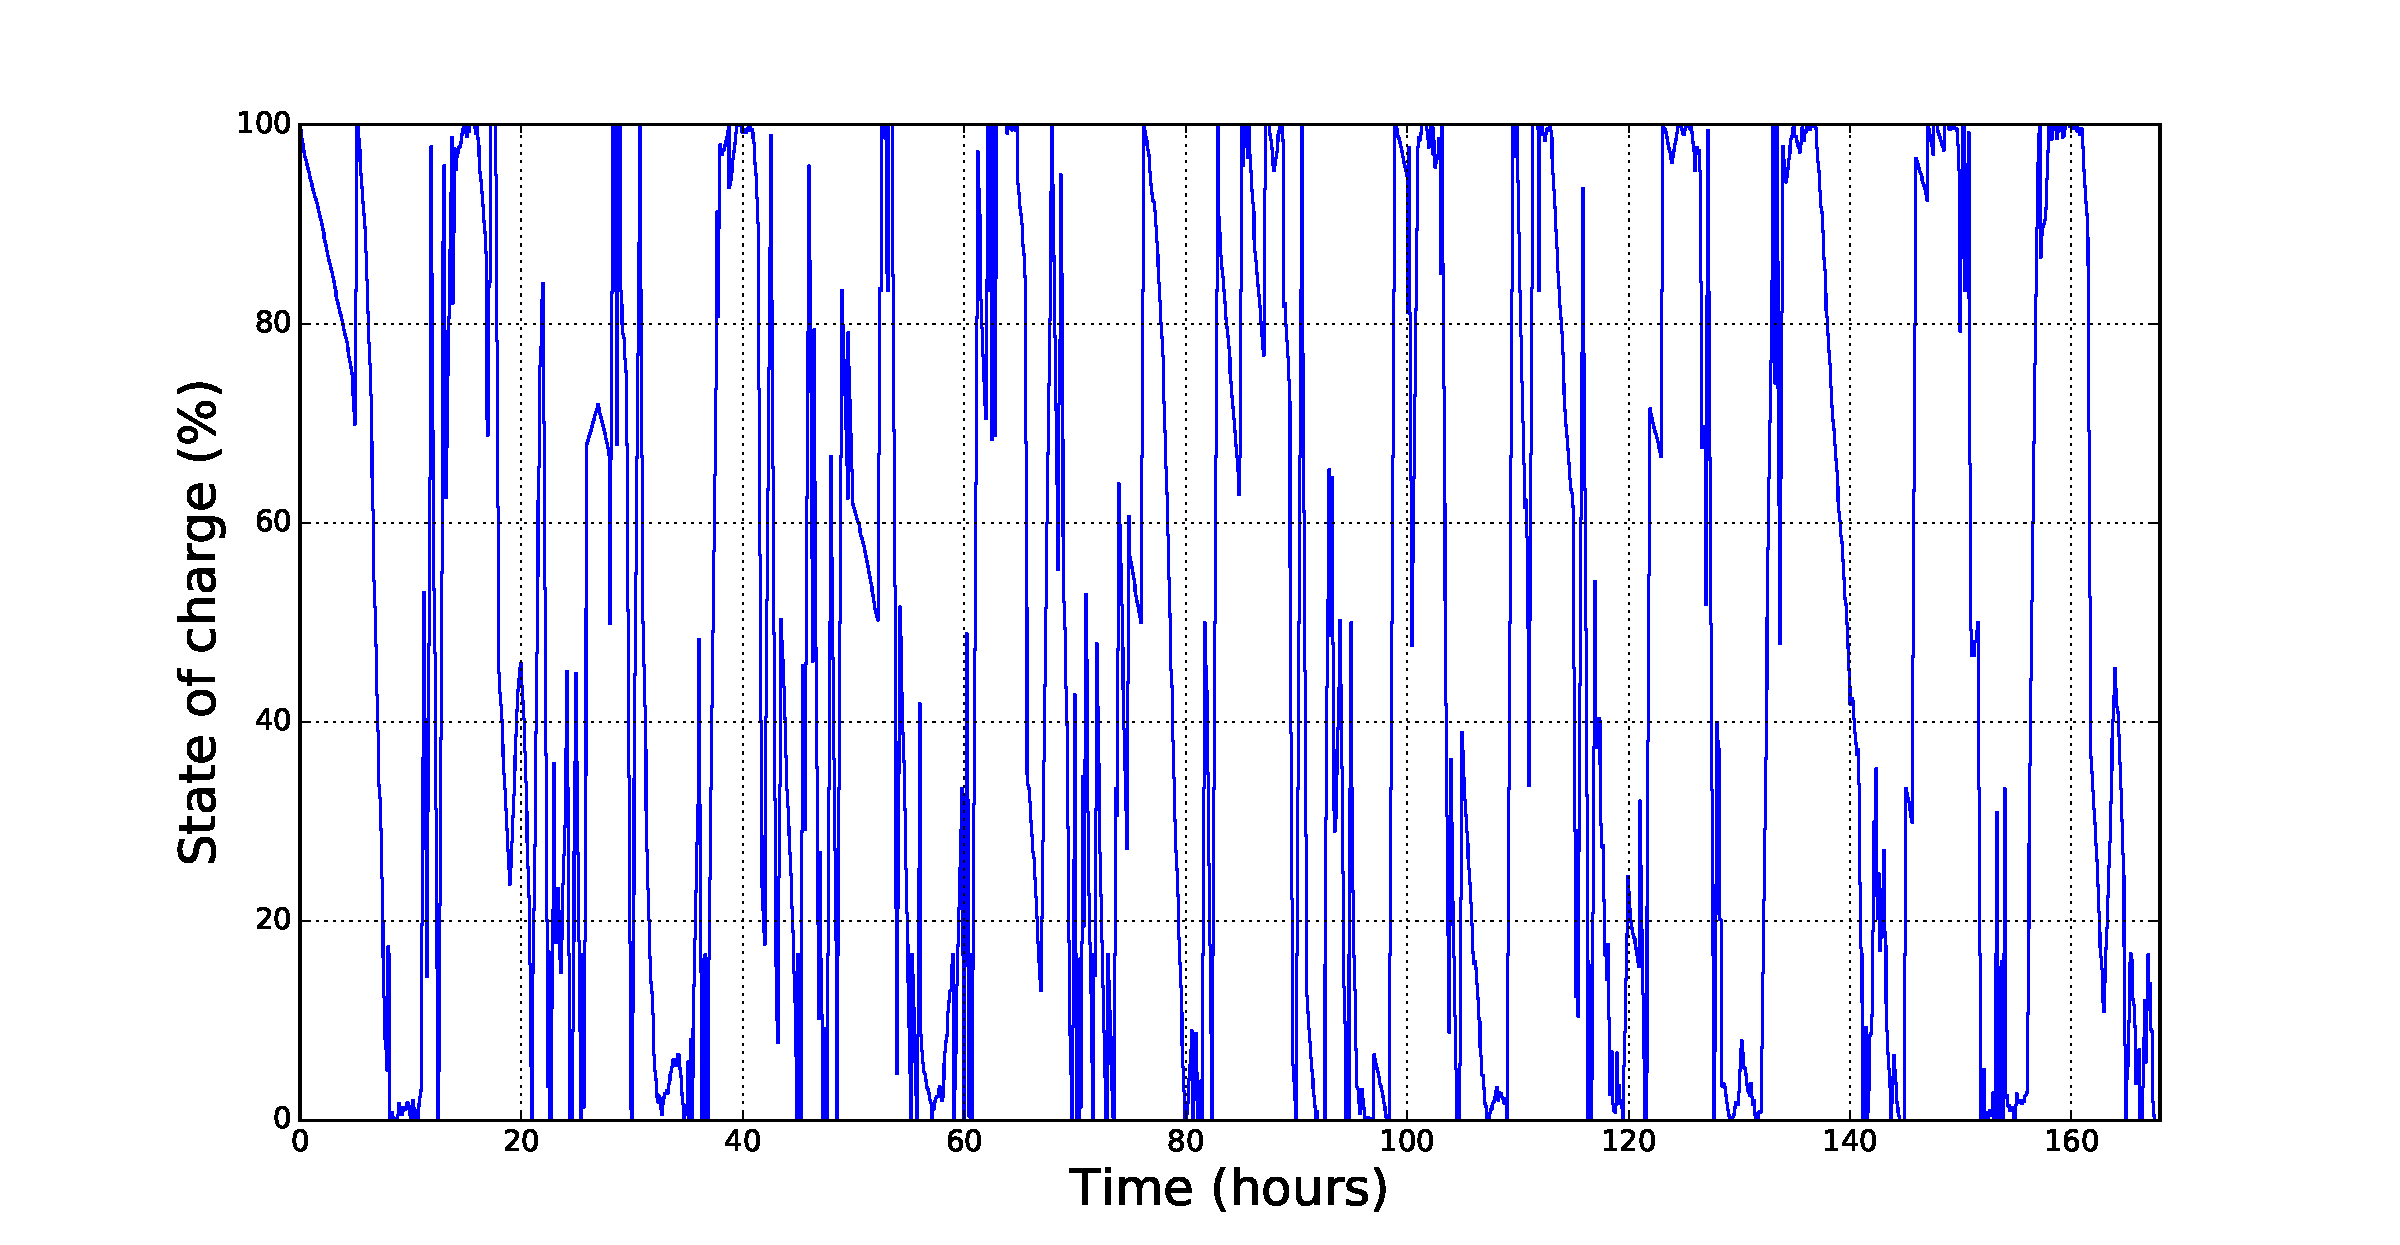
\includegraphics[width=0.7\textwidth]{Figures/Plots/fullproblem_stoch/soc_fp_st.pdf} \caption{State of charge trajectory}\label{fig:soc_fp_st}
\end{subfigure}
\caption{Operating condition of battery when participating in both day-ahead and real-time markets}
\end{figure}
%\FloatBarrier
Thus market participation in both timescales is important for maximizing the economic potential. The typical problem in a stochastic setting (considering only 50 samples of load scenarios) for 1 week planning consists of 520900 variables, 722500 linear constraints, and takes Gurobi 35-40 seconds to solve it. 
If the number of scenarios is increased, the problem size would grow exponentially. While on increasing the planning period the problem size increases linearly. Therefore, for problems involving simultaneous participation in both real-time and day-ahead markets, we use sample average approximations and some relaxations to estimate the bounds on the expected revenues that can be earned. For the same kind of problems we use advanced techniques for solving stochastic programming problems in Section \ref{subsec:dual} and we compare their performance with respect to solution time and the expected revenue obtained.

\subsubsection{Bounds on Sample Average Approximation}\label{subsec:sampleavg}
To estimate a confidence interval bound on the expected revenue from market participation at both timescales, we sample 100 different sets (or batches) of 50 random paths (realizations of load profiles over 168 hours) along the scenario tree. We solve the two-stage approximation of the extensive form problem with each of these 100 different sets of 50 sample paths from the scenario tree and obtain the expected value over the 100 batches of the optimal revenues of operating the battery in the setting described in \ref{subsec:opt_unc}. This expected optimal revenue over 100 batches provides a statistical lower bound of the actual optimal cost that would be obtained if we were to solve the stochastic program for the complete scenario tree. We can then obtain a confidence interval of the expected revenue by using the student's t-distribution. The confidence interval on this statistical lower bound can be tightened by taking a greater batch size. 

With 100 batches of 50 random paths, the expected optimal revenue is \$709.74 with a 95\% confidence interval of [\$709.39,\$710.08]. We observe that the expected optimal revenue over 100 different batches is quite close to the expected revenue that we obtained for a single set of 50 random paths in Section \ref{subsec:economic}, which is \$711.08 with the difference being only 0.19\%. 

The approximate problem by sampling 50 paths from the scenario tree is typically solved in 35-40 seconds in Gurobi. Thus, the problem with full scenario tree can be approximated very efficiently by sampling a limited number of paths and solving the obtained problem of smaller size.

With the same sampled set of 50 paths evaluated in Section \ref{subsec:economic}, for which the expected revenue is \$711.08, we compare the various bounds on the expected revenue obtained by the following relaxations/approximations of the problem: 
\begin{itemize}
\item \textbf{Bound from Mean-Value Problem}\\
In the mean-value problem, we assume that at every hour only the mean of the possible scenarios of load profiles will realize. We obtain a market participation policy for the battery-building system by solving a deterministic optimization problem with this assumption. We then implement this 'mean-value policy' in various possible scenarios for load profiles and evaluate the expected revenue over all scenarios. The expected revenue from the mean-value policy is bound to be less than that from the 'stochastic policy' because the mean-value policy does not consider all possible scenarios while solving the optimization problem. Hence, the expected revenue from the mean-value policy is a lower bound on the expected revenue from the stochastic policy (or an upper bound on expected cost). 

The expected revenue from the mean-value policy is \$697.61 which is about 1.9\% less than that from the stochastic policy (Table \ref{tab:bounds}). Thus, the value of stochastic solution, in this case, comes out to be \$13.47. The major benefit of the stochastic policy can be observed from Figure \ref{fig:histogram}. We can see from Figure \ref{fig:histogram} that the stochastic policy protects us from getting very low revenues in some scenarios compared to the mean-value policy. Also, the distribution of revenues in various scenarios is shifted towards higher value for the stochastic policy than the mean-value policy.

\item \textbf{Bound with Perfect Information:}\\
To find the bound with perfect information, we assume that we had perfect information (or accurate prediction) of all the possible scenarios of load profiles. Thus, we can solve a deterministic optimization problem for each of the scenarios separately and obtain a market participation policy and revenue for the battery-building system for each scenario. The expected value of the revenues obtained for all scenarios gives us an upper bound on the expected revenue from the stochastic policy (or a lower bound on expected cost) because with perfect information of each scenario we are able to plan the best policy for each scenario.

The expected revenue from all the perfect information policies is \$714.18 which is about 0.44\% greater than that from the stochastic policy (Table \ref{tab:bounds}). Thus, the value of perfect information is \$3.10 for chosen set of 50 paths. From Figure \ref{fig:histogram} we observe that the revenues in perfect information case are all greater than all other policies showing the value of having perfect information. However, the stochastic policy does not achieve far worse expected revenues and it emphasizes that stochastic policy is better when we do not have perfect information for the random data. 

\item \textbf{Bound with Restriction on State Variables}\\
This approach gives a better lower bound on the expected revenue from the stochastic policy. We add a restriction on the state variables (the energy level of the battery) at each stage (hour) to be a first-stage decision. This means that require that the values of the energy levels of the battery at the end of every hour in the planning period are to be decided before observing any uncertainty and in real-time (every 5-minute subinterval) the energy level of the battery needs to follow a trajectory so that it gets to the already decided values at the end of every hour. This gives us an approximation of the stochastic program where we just have an added restriction. Hence, solving this problem will give a lower bound on the expected revenue.

The stochastic program with restriction on state variables gives an expected revenue \$698.92 which is 1.71\% less than that from the stochastic policy (Table \ref{tab:bounds}), while 0.19\% higher than that from the mean-value policy. Thus, we get an improved lower bound on the expected revenue (or upper bound on expected cost) from this approach. The major benefit of the stochastic policy can be observed from Figure \ref{fig:histogram}. We can observe in Figure \ref{fig:histogram} that the problem with restriction on states does slightly better than mean-value policy in terms of protecting us from scenarios with very low revenue, but it is possible in a few scenarios that the mean-value policy performs better that the policy with restriction on states. The stochastic policy achieves better distribution of revenues that the restricted state case because the stochastic policy has no restriction on state variables.
\end{itemize}
\begin{figure}[h!]
\begin{center}
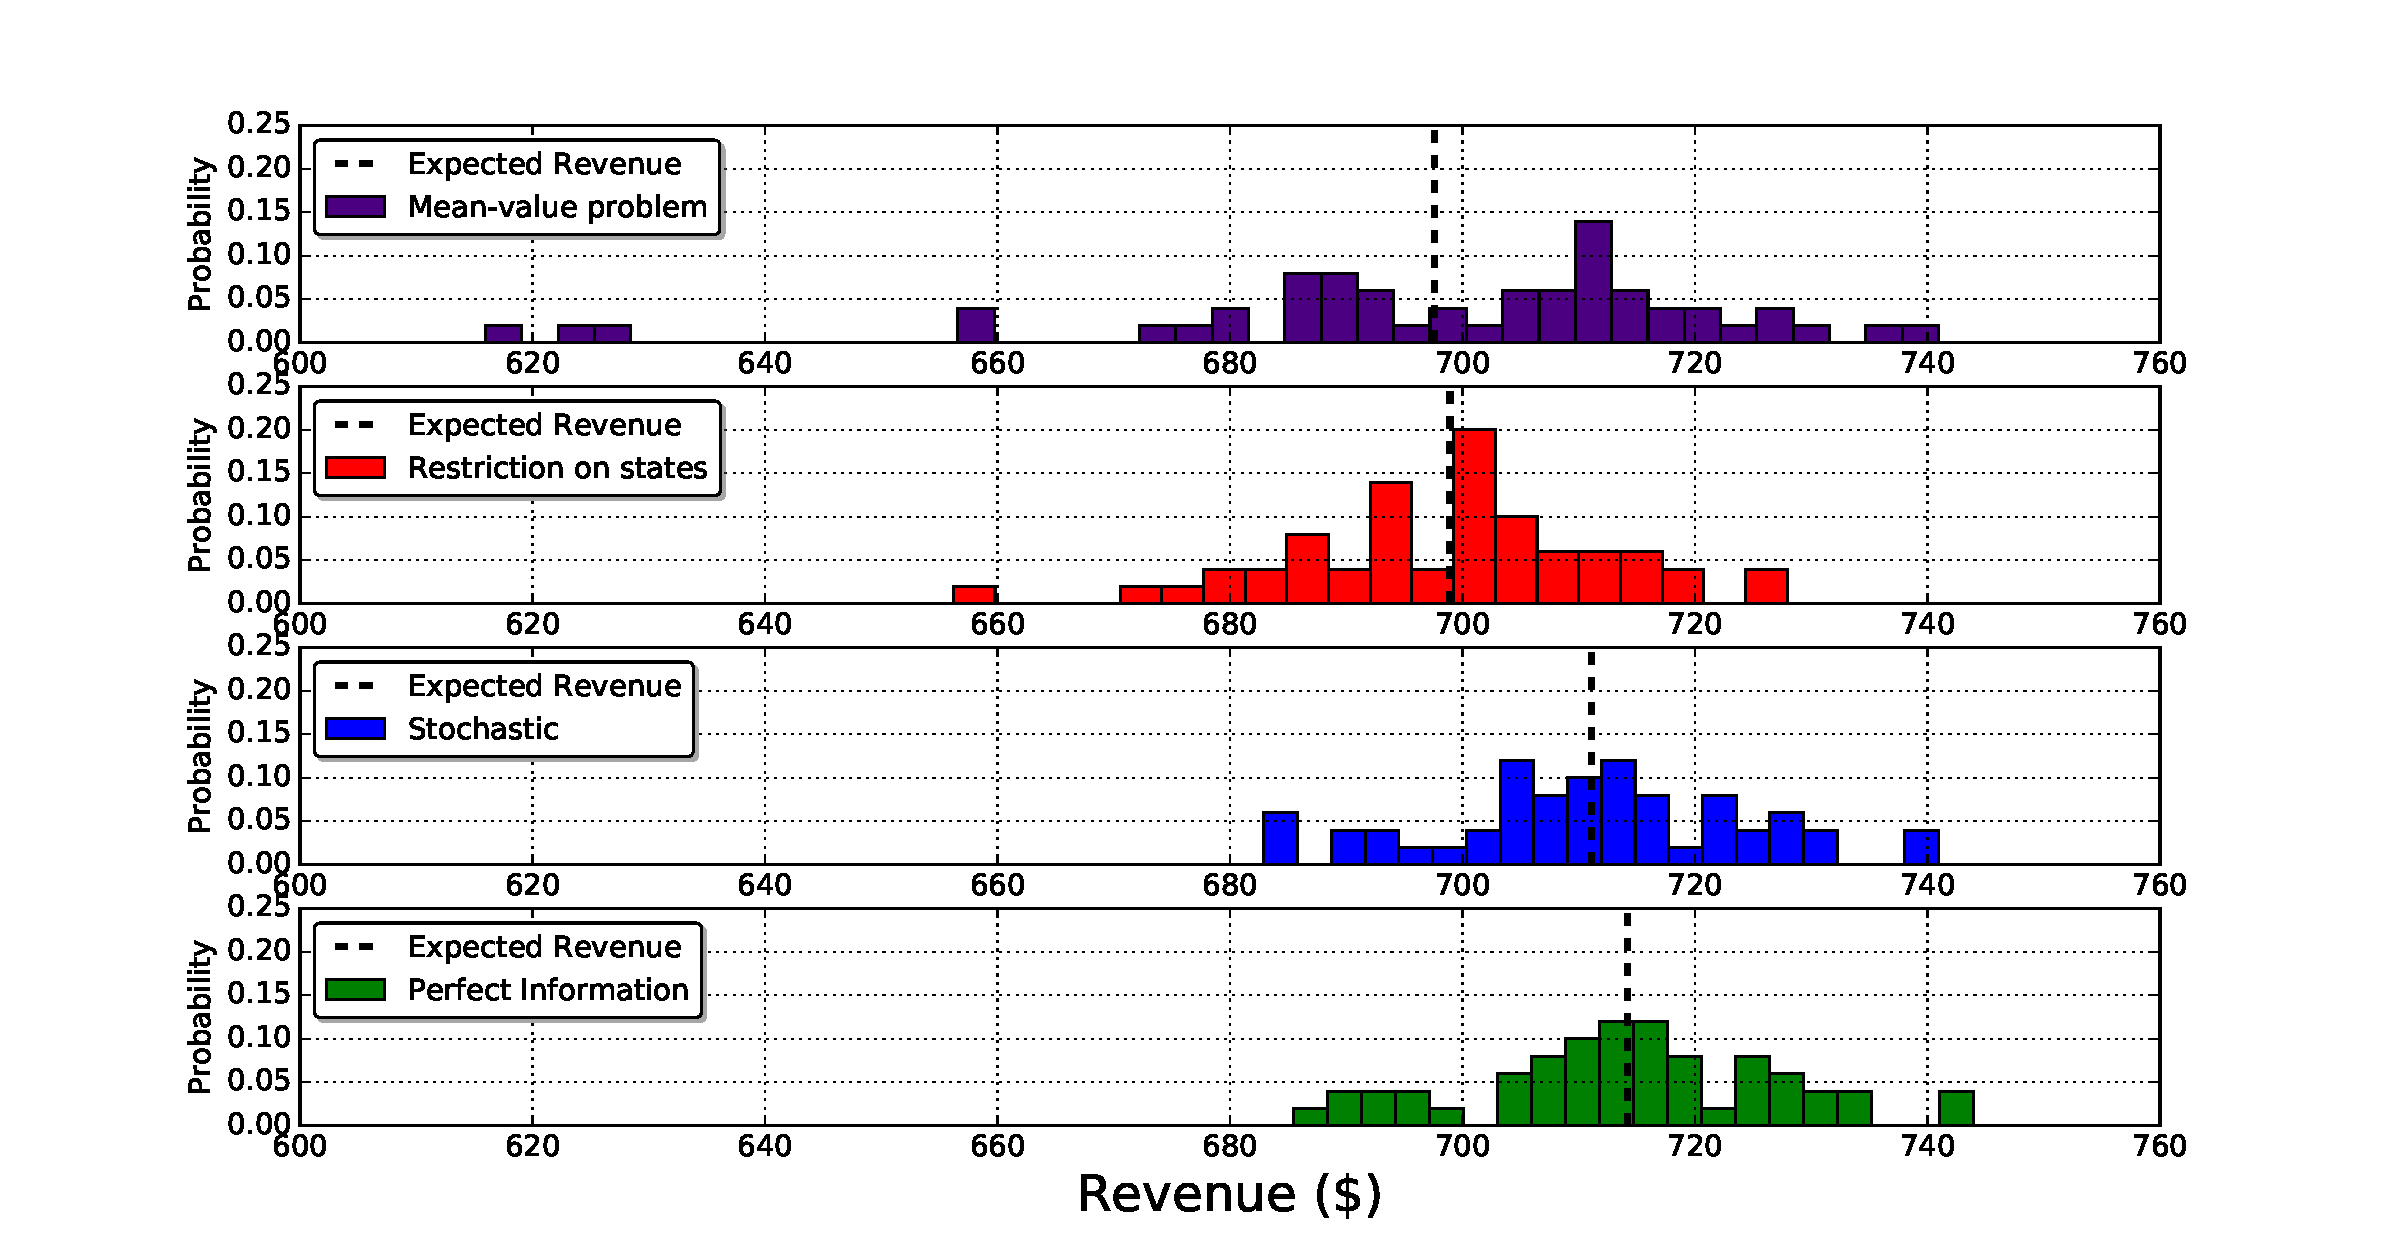
\includegraphics[scale=0.42]
{Figures/Plots/fullproblem_stoch/histogram_costs.pdf} \caption{Distribution of revenues for a set of 50 sample scenarios (paths) of load profiles for a week's planning period. The policy from the perfect information solution gives a distribution of revenues which is populated towards higher value. The policy from the extensive form of stochastic program with the same sample scenarios achieves better expected revenues as compared to the cases with restriction on state variables and the mean-value approximation.
}\label{fig:histogram}\end{center}
\end{figure}
\FloatBarrier
\begin{table}[!ht]\centering
\caption{Expected Revenue from Different Problems to Estimate Bounds}
\begin{tabular}{|C{5cm}|C{3.5cm}|C{3.5cm}|} 
\hline 
Problem  & Expected Revenue (\$) & \% Gap from Stochastic Policy \\
\hline 
Mean-value & \$697.61 & -1.9\%\\ 
\hline 
Restriction on state variables & \$698.92 & -1.71\% \\ 
\hline 
Stochastic (extensive form) & \$711.08 & 0\% \\ 
\hline 
Perfect information & \$714.18 & +0.44\% \\ 
\hline 
\end{tabular} \label{tab:bounds} 
\end{table}

\subsection{Multi-Stage Approaches}\label{sec:multistage}
\subsubsection{Stochastic Dual Dynamic Programming} \label{subsec:dual}
Our state variable $E_{i,k}$ (energy-level of battery at any time) captures the history of load demands realized and the decisions made in the previous stages; thus providing stage-wise independent scenario realizations. The stochastic dual dynamic programming (SDDP) is applicable in this case. 

The stochastic problem at each node is for making the energy commitment decisions from that hour to the next hour i.e we formulate a problem for decisions in future (where we have not yet observed any realizations). This is because we only have samples of scenarios for that future hour and not the perfect information. To get a lower bound, we have to the solve the problem at root node at which the realized scenario for random data has to be known. In our case we consider the root node problem to be the stochastic program between t = -1 hr and 0 hr. Since we are not participating before t = 0 hr, we know that the random data (load in our case) is 0 between t = -1 hr and t = 0 hr (Figure \ref{fig:scenario_tree}). Hence, the stochastic program at our root node is minimizing the $\theta_{1}$ variable (capturing the future costs), such that $\theta_{1} \geq \underline{\theta}$. The solution to this gives a starting lower bound. We give a lower limit $\underline{\theta}$ for $\theta_1$ because our cost is negative since we are maximizing revenue (or minimizing negative revenue). In the case of the root node, just $\theta_1$ is being minimized, which becomes unbounded. Thus we need to provide an initial lower bound for $\theta_1$. $\underline{\theta}$ is found by assuming energy market participation with a full capacity of the battery in both markets for the full planning period i.e. for negative electricity prices, battery participates in full negative capacity (buying power) and for positive prices, it sells power at full capacity. Thus at the root node, $\theta_1$ will be the maximum revenue that is achievable without any constraints on battery storage capacity.   

In our multi-scale problem, the state variables ($E_{i,k}$) are defined at 12 sub-intervals (of 5 minutes each) within a stage. In standard (one timescale) SDDP algorithm, we take dual of the constraint linking the state variable at the current stage to the state variable at the previous stage. This does not work in case of multi-scale problems since the state variables vary at a timescale of 5 minutes within a stage, while the stages are realized at every one hour. The value of the state variable that is carried forward to the next stage is only the state at the last sub-interval of the current stage i.e the state variables are linked within each sub-intervals and not directly between the stages. We therefore use the sum of duals of the constraints inter-linking these state variables at all sub-intervals within the stage; this sum in effect links the final value of the state variables between consecutive stages. With this modified approach we implement our version of the SDDP algorithm (for a planning period of $T_{P}$ hrs) as follows:    
\emph{
\begin{enumerate}
\item Set iteration counter $i = 1$. Generate a compact scenario tree with 50 nodes at every stage ($T_{P}$ stages in total).
\item Formulate the root node problem (k=0) as described above. Denote this optimization problem by $\mathcal{P}^f_{0}$.\\\\
\textbf{Forward Pass:}
\item Solve the optimization problem $\mathcal{P}^f_{0}$ and get $\theta_1$. Set the current lower bound, $lb = \theta_1$. Set $k = 1$.
\item Sample a load profile for stage $k$. 
\item \emph{If} $i>1$,\\ go to Step 6, \\ \emph{else},\\ formulate an optimization problem as described in Section \ref{subsec:deterministic}, with $n_\text{dam} = k$, $ E_{0, k} = E_{n_\text{rtm}, k-1}$ and using the loads sampled in Step 4. Modify the original objective function (say, $f_{k,i}$) by adding a $\theta_{k+1}$ (capturing future costs) variable (bounded below by $\underline{\theta}$). Denote the resulting optimization problem by $\mathcal{P}^f_{k}$.
\item Solve the optimization problem $\mathcal{P}^f_{k}$, get $E_{n_\text{rtm}, k}$ and $f_{k,i}$. Set $k = k +1$. 
\item \emph{If} $k <= T_{P}$, go to Step 4 \emph{else} go to Step 8 and set $k = T_{P}$.
\item Set current upper bound, $ub = \frac{1}{i}\sum\limits_{p = 1}^{i}\sum\limits_{k \in \mathcal{T_D}}{f_{k,p}}$ \\\\
\textbf{Backward Pass:}
\item Set $\overline{v}^i_{k+1} = 0, \overline{\rho}_{k+1} = 0$.
\item \emph{for $s = 1,2,....,N$}
\begin{enumerate} 
\item \emph{If} $i>1$,\\ go to Step (b), \\ \emph{else},\\ formulate a scenario subproblem for scenario $s$, as described in Section \ref{subsec:deterministic}, with $n_\text{dam} = k$, $E_{0, k} = E_{n_\text{rtm}, k-1}$ (obtained from forward pass) and using the loads in scenario $s$. Modify the original objective function (say, $f^b_{k,i}$) by adding a $\theta_{k+1}$ (capturing future costs) variable (bounded below by $\underline{\theta}$) and denote the modified objective function by $Q^{i+1}_{s,k+1}(E_{0, k})$. Denote the resulting optimization problem by $\mathcal{P}^b_{k}$. 
\item Add a cut to the optimization problems $\mathcal{P}^f_{k}$ and $\mathcal{P}^b_{k}$: $\theta_{k+1} \geq \overline{v}^i_{k+1} - \overline{\rho}_{k+1}E_{n_\text{rtm}, k}$
\item Solve the problem $\mathcal{P}^b_{k}$. Get the optimal objective value $Q^{i+1}_{s,k+1}(E_{0, k})$ and the duals corresponding to each of the ${n_\text{rtm}}$ constraints linking the state variables at each subinterval. Denote the sum of these duals by $\rho_{s,k+1}$ and calculate $v^i_{s,k+1} = Q^{i+1}_{s,k+1}(E_{0, k}) - \rho_{s,k+1} E_{n_\text{rtm},k-1}$
\end{enumerate}
\emph{end for}
\item $\overline{v}^i_{k+1} = \frac{1}{N}\sum\limits_{s=1}^{N}{v^i_{s,k+1}}, \quad \overline{\rho}_{k+1} = \frac{1}{N}\sum\limits_{s=1}^{N}{\rho_{s,k+1}}$. Set $k=k-1$
\item \emph{If} $k >= 1$, go to Step 10, \emph{else if} $ub - lb \geq \epsilon$, go to Step 3, \emph{else}, STOP.
\end{enumerate}}

We implement the SDDP algorithm described above on the battery-building system participating for one week in the 2-timescale electricity markets. We use the same set of 50 sampled scenarios for load profiles for the full week as in \ref{subsec:economic}. We solve all the forward pass problems and scenario subproblems in the backward pass using Gurobi. For a typical run of the SDDP algorithm, we obtain the following performance of the algorithm and the upper and lower bounds at convergence with a tolerance limit $\epsilon = 0.1$:
\begin{itemize}
\item Number of iterations to converge: 221
\item Time taken to converge: 825.8 sec
\item Final lower bound on cost (Equation \ref{objective_unc}): -554.88
\item Final upper bound on cost (Equation \ref{objective_unc}): -554.79 with a confidence interval of [-554.57, -555.02]
\end{itemize}

The trajectory obtained for the lower bounds and the upper bounds with its confidence interval at every iteration in a typical SDDP run is shown in Figure \ref{fig:bounds}. As the number of iterations increases the upper bound comes closer to the lower bound with its confidence interval shrinking. This convergence behaviour shows that the modification that we made to the standard SDDP for our multi-scale problem is valid. 
\begin{figure}[h!]
\begin{center}
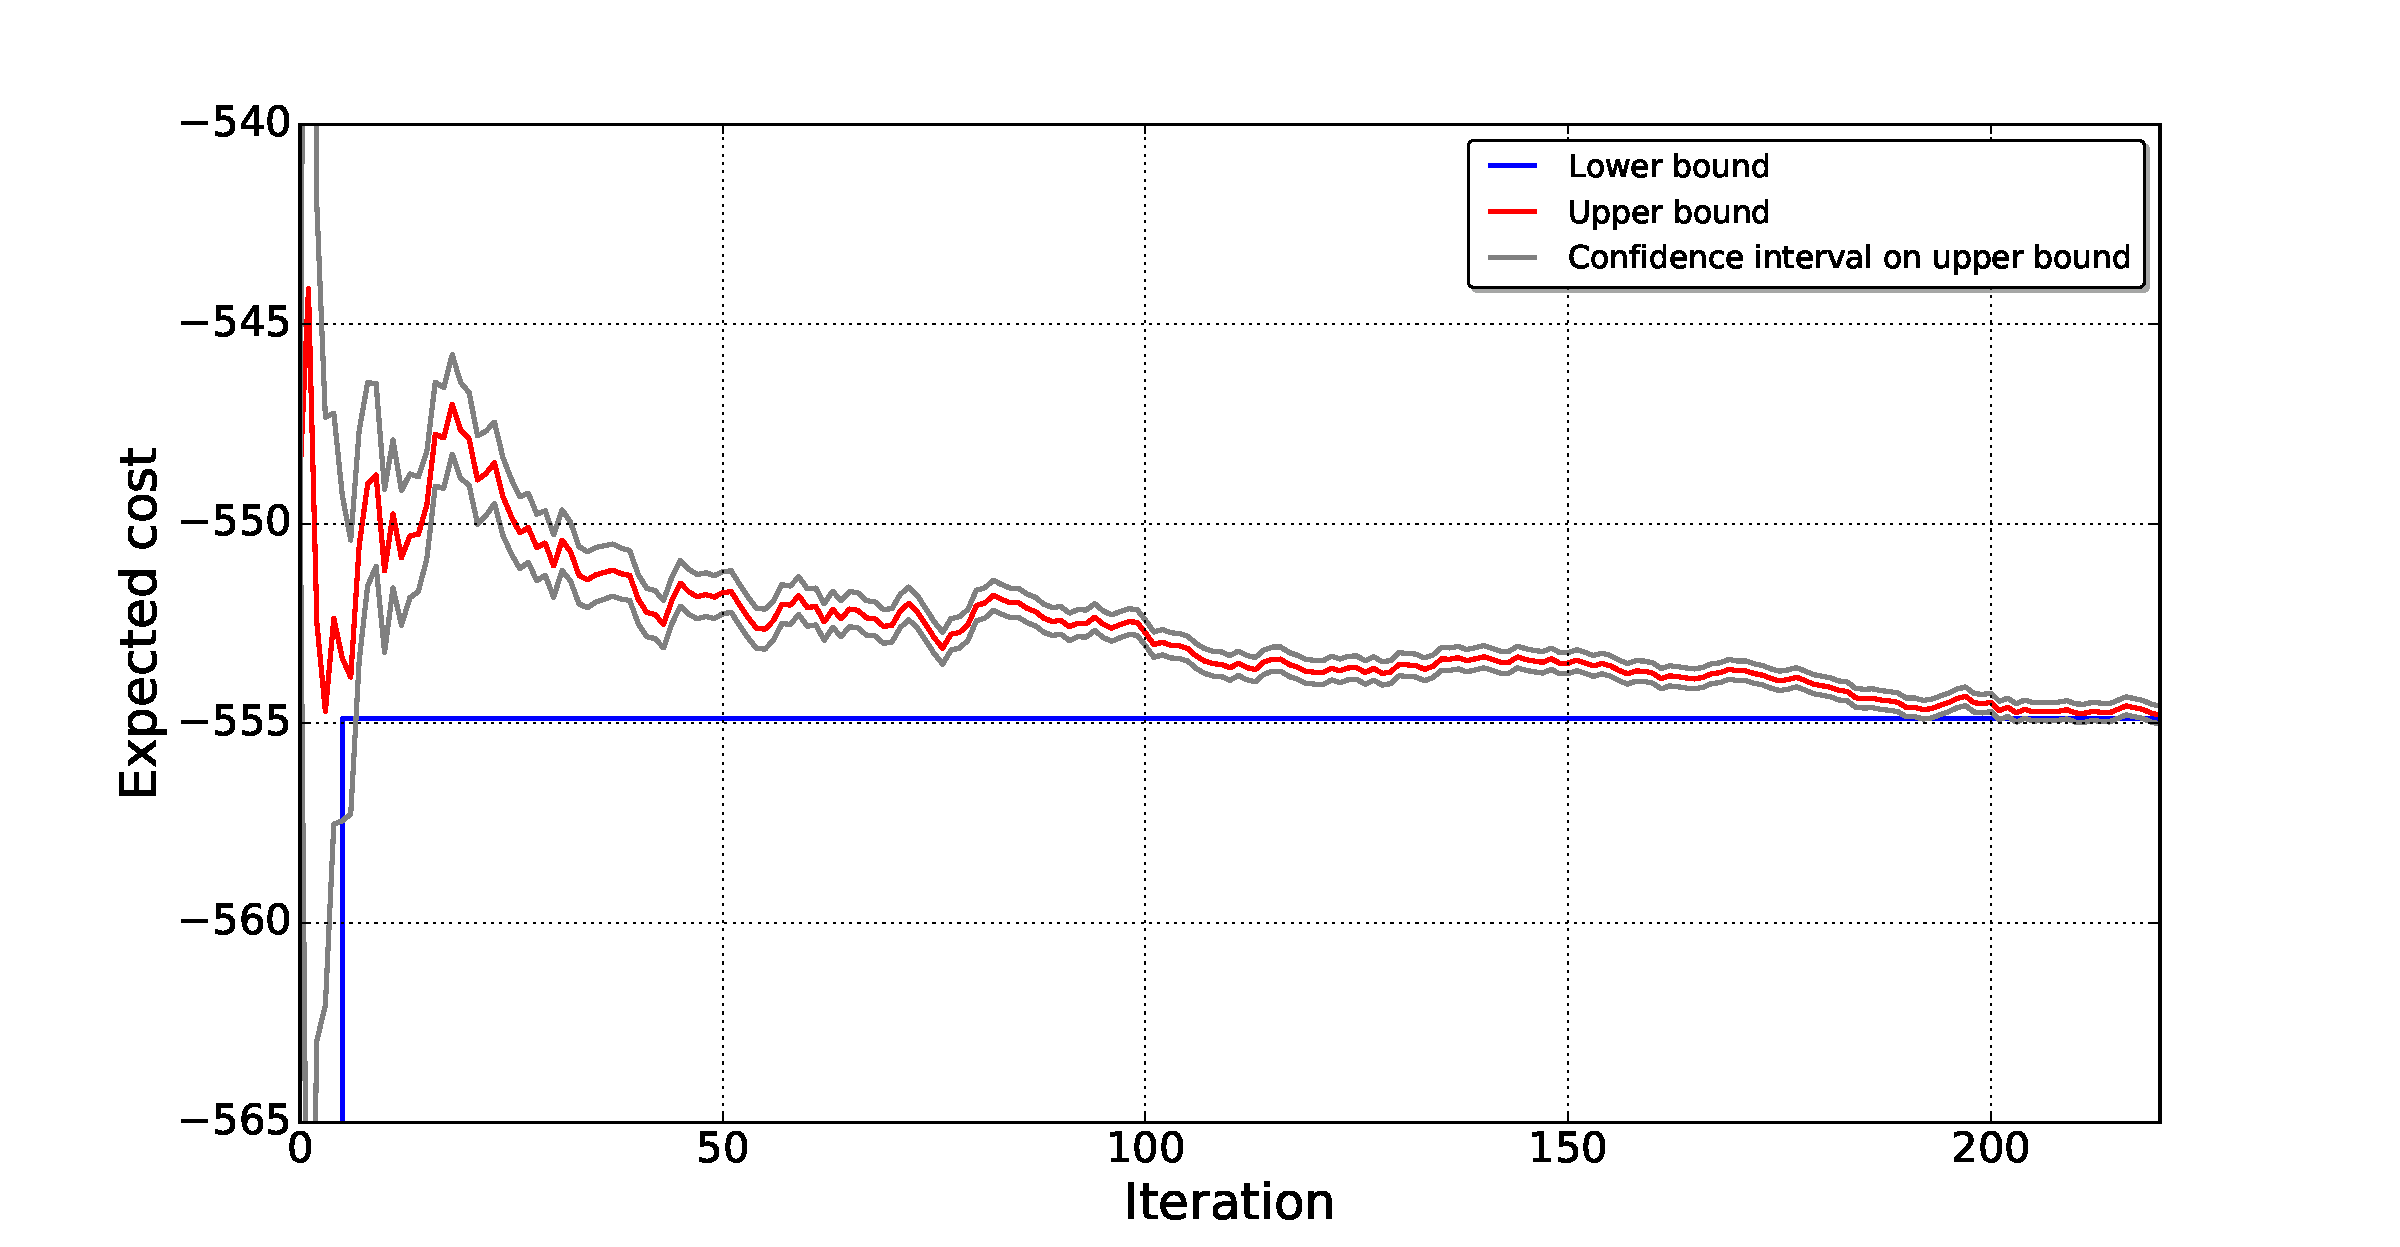
\includegraphics[scale=0.4]
{Figures/Plots/dualdynamic/bounds.pdf} \caption{Trajectory of the lower and upper bounds obtained at every iteration of stochastic dual dynamic programming}\label{fig:bounds}
\end{center}
\end{figure}
\FloatBarrier
The optimal revenue obtained from SDDP is about \$554.84 (taking the average of the final upper and lower bounds), which is significantly less than the values obtained from the two-stage approximations. This is due to the fact that the SDDP algorithm does not make the two-stage approximation. In every iteration, it solves the problem along different paths in the scenario tree performing stage-wise forward pass, while in backward pass it solves all scenario subproblems within a stage and transfers that information to the forward pass in the form of cuts generated using the duals. Thus, the SDDP efficiently evaluates the cost in a large number of paths in the tree and is a much closer approximation to the multi-stage problem. Hence, the optimal cost obtained from the SDDP algorithm provides a better lower bound on the true optimal cost of the full multi-stage problem.
\FloatBarrier
\subsection{Receding Horizon Scheme}
In practical situations, we may not have the sample scenarios for load profiles available for the full week or a longer planning period that we want to schedule our market participation policy for. In situations when we have the profiles for load scenarios are available for fewer time periods, a receding horizon scheme is useful and can be implemented to minimize the cost looking at only that much ahead in future for which we have the sample load scenarios. The receding horizon scheme is expected to do worse than the case when we have sample scenarios for load profiles available for the full planning period, but it still outperforms a policy obtained using mean-value counterpart in the same situation (when we have information available for less period of time in future). 

We assume that at every hour $\tau$, we have a set of samples for the scenarios for load profiles available only for the next $T$ hours while we want to plan for a planning period $T_{P}$ hrs. At $\tau$, we can solve a stochastic program $\mathcal{P}_{\tau}$, where $\mathcal{P}_{\tau}$ is the extensive form of the stochastic program described in Section \ref{subsec:opt_unc} with $n_\text{dam} = T$. To solve this stochastic program, it requires the inputs $L_{i,k,s}$, $\pi_{i,k}$ and $\pi_k$ $\forall i \in \mathcal{T_R}, k \in \{\tau+1, ..., \tau+T\}, s \in \mathcal{S}$ and the initial energy level of the battery at that hour $\tau$, $E_{\tau}$. For compact representation, let $L_{\tau}(\xi_{\tau})$ denote the set of load profiles in all scenarios for future $T$ hours and $\pi_{\tau}$ be the set of prices in day-ahead and real-time markets for hour $\tau+1$ to $\tau+T$. We can now solve the $T$-hour horizon stochastic program $\mathcal{P}_{\tau}\left(E_{\tau}, \pi_{\tau}, L_{\tau}(\xi_{\tau})\right)$.

The receding horizon scheme which we implement on the building-battery system is described below.
\emph{
\begin{enumerate}
\item Consider $\tau = 0$.
\item With $E_\tau$, $L_{\tau}(\xi_{\tau})$ and $\pi_{\tau}$, solve the stochastic program $\mathcal{P}_{\tau}\left(E_{\tau}, \pi_{\tau}, L_{\tau}(\xi_{\tau})\right)$ over a $T$-hour horizon.
\item By solving $\mathcal{P}_{\tau}\left(E_{\tau}, \pi_{\tau}, L_{\tau}(\xi_{\tau})\right)$, obtain a profile for net battery discharge, $P_{net}$, between hours $\tau$ and $\tau+1$ corresponding to each scenario of load profile in the interval.
\item Using a realized scenario for load (random) between hours $\tau$ and $\tau+1$, evolve battery storage level to $E_{\tau+1}$.
\item Set $\tau = \tau+1$.
\item If $\tau = T_P$, then stop, else go to step 2.
\end{enumerate}
}

We implement the receding horizon scheme to plan a market participation policy for the battery-building system participating in both the real-time and day-ahead electricity markets. We use a horizon of $T=24$ hours, i.e. at any hour we have a sample set of scenarios of load profiles for only next 24 hours. We simulate the receding horizon scheme using the same set of 50 sampled scenarios for load profiles for one week as in \ref{subsec:economic}. However, to simulate the receding horizon up to 7 days, we need to generate additional sample scenarios for the $8^{th}$ day because after the simulation reaches the last day of the week, it formulates the optimization problem with the loads of next 24 hours which goes beyond the $7^{th}$ day. So, we generate the additional samples of load profiles using the method described in Section \ref{sec:setting} and use these as the scenarios for loads in $8{th}$ day. At the end of the simulation, we evaluate the revenue from the obtained policy. We repeat the simulation with 50 different paths of load realizations at every hour and get an approximation of the expected revenue and a confidence interval on the same.

By implementing the above procedure, the expected revenue from the policies for 50 different paths is \$697.64 with a 95\% confidence interval of [693.95, 701.35]. 
Gurobi takes less than 2 seconds (1.3-1.7 sec) to solve the 24-hour horizon problem at every stage. So, the complete simulation for a week can be performed in about 5 minutes. The problem that Gurobi solves at every stage in the receding horizon simulation with 24-hour horizon consists of 117650 linear constraints and 88850 variables, which is of much smaller than the problem for full 1 week (Section \ref{subsec:economic}).

The expected revenue from the receding horizon simulations is only about 0.2\% less than that obtained from the two-stage approximations in Section \ref{subsec:sampleavg}. This indicates that implementing the policy for only the next hour, updating the state variable and re-optimizing the system for the next 24 hours at every stage helps in carrying minimizing the impact of having sample profiles of loads for a lesser period. The receding horizon scheme implements a two-stage approximation at every stage. Also, near the end of the planning period, the 24-hour horizon problem (at every step) considers loads and prices of the day beyond the planning period (7 days). This gives the system more flexibility in terms of planning an optimal policy for those hours. Therefore, the expected revenue from receding horizon simulations is closer to that in \ref{subsec:sampleavg} than that obtained from stochastic dual dynamic programming (\ref{subsec:dual} which is a multi-stage implementation.

\section{Conclusions}
From our study of various revenues generated by the participation of a battery-building system in different timescales of electricity markets, we conclude that the simultaneous participation in both real-time and day-ahead markets is much more profitable as compared to participation in the market at only one timescale alone. The decision-making for market participation involves forecasting of loads and that introduces uncertainty in the problem. So, stochastic optimization techniques need to be used to determine the optimal participation policy over a planning period. The typical stochastic programs in extensive form for participation in both markets for one week period and assuming 50 scenarios for the uncertain loads at every stage involve over 0.5 million variables and over 0.7 million constraints. The optimization problem can easily become intractable if we consider a greater number of scenarios at every stage. 

So, two-stage approximation and sample average approximation become useful to estimate bounds on the optimal revenue. Techniques to solve multi-stage stochastic programs like the stochastic dual dynamic programming can estimate a much realistic estimate of the expected revenue by efficiently solving the problem at many more number of nodes without taking two-stage approximation. Since the SDDP solves very small linear programs, although many of them, in every iteration, it can be very efficient in solving with even larger number of scenarios. Receding horizon scheme can be very effective in situations where we do not have the scenarios for the random load data available for the full planning period. The receding horizon gives a policy that generates almost the same expected revenue as that obtained by a policy from the solution of extensive form stochastic program.

A comparison of problem size that Gurobi has to solve at every stage and iteration in each of the methods studied is summarized in Table \ref{tab:comparison}. 
\begin{table}[!ht]
\centering
\caption{Problem sizes and time taken by Gurobi to solve corresponding individual problems in different methods for 1 week planning}
\begin{tabular}{|C{3cm}|C{2cm}|C{2.5cm}|C{2.5cm}|C{3.5cm}|}  
%\begin{tabular}{|c|c|c|c|c|}  
\hline 
\multirow{2}{*}{Method} & \multirow{2}{*}{\parbox{2cm}{\centering Expected Revenue (\$)}} & \multicolumn{2}{C{3cm}|}{\parbox{5cm}{\centering Individual problem sizes at every stage and iteration }} & \multirow{2}{*}{\parbox{3.5cm}{\centering Time taken to solve the individual problem}}\\
\cline{3-4}
  &  &   Variables  &  Constraints & \\[0.5cm]
\hline 
Two-stage approximation & 711.08 & 520,900 & 722,500 & 35-40 sec \\ 
\hline 
Stochastic dual dynamic programming  & 554.84    & 65 & 88  & $<$0.01 sec \\ 
\hline 
Receding horizon & 697.64 & 88,850 & 117,650  & $<$2 sec \\ 
\hline 
\end{tabular} \label{tab:comparison} 
\end{table}
\FloatBarrier

\section{Future Work}
\subsection{Price Uncertainty}
Future direction of this work can be to investigate the effect of price uncertainty on the expected revenue. With the optimization model developed for the system, it will be an easy extension to include uncertainty in the electricity prices. Similar to the loads, uncertainty in prices can be captured by a set of possible profiles for the price signals. The stochastic program will now become larger due to the introduction of uncertainty in prices; the total number of possible scenarios of uncertainty will now be a product of the number of scenarios of each of the random data, i.e. loads and prices. In such a case, the number of samples in the sample average approximations would have to be much higher to get a good estimate of the optimal revenue. We can also investigate how the advanced techniques like SDDP perform in such problems. The problem size can be brought down by considering loads and electricity prices to be correlated so that a scenario corresponds to a realization loads and prices together.
\subsection{Three Layer Markets}
We can also investigate the revenue potential of participating in a three timescale market. Participating in a three layer market can provide more flexibility of generating higher revenues. The third timescale in California ISO operates at 15-minute intervals and is also categorized under the real-time market. So the market decisions for this timescale are also recourse decisions. So, the problem size will grow with the addition of decision variables for that timescale in each scenario. A study of the performance of different methods can be carried out for the three level market under uncertainty. Because the problem size is bigger, it might be more practical to solve the stochastic program using a receding horizon scheme with a shorter horizon to make the problem tractable in real-time.


\bibliography{cs719}

\end{document}
